\documentclass[11pt,a4paper]{article}
\usepackage[margin=22mm]{geometry}
\usepackage{fontspec}
\setmainfont{Latin Modern Roman}
\setsansfont{Latin Modern Sans}
\setmonofont{Latin Modern Mono}
\usepackage{amsmath,amssymb}
\usepackage{unicode-math}
\setmathfont{Latin Modern Math}
\usepackage{longtable,array,fvextra,adjustbox,needspace}
\usepackage{pgfplots}
\usepackage{pdflscape}
\pgfplotsset{compat=1.18}
\usepackage[colorlinks=true,linkcolor=blue,urlcolor=blue,unicode=true]{hyperref}
\usepackage{xurl}
\newcounter{listing}
\newcounter{scripttable}
\definecolor{pcd1}{HTML}{005A78}
\definecolor{pcd2}{HTML}{6B2CB1}
\definecolor{pcd3}{HTML}{447766}
\definecolor{pcd4}{HTML}{9A3E20}
\definecolor{pcd5}{HTML}{756000}
\setlength{\parindent}{0pt}
\setlength{\parskip}{0.65em}
\setlength{\emergencystretch}{3em}
\begin{document}
\hypersetup{pdftitle={Variation connects repeated measurements with uncertainty},pdfsubject={Authored thematic script},pdfcreator={Project Chemie Digital LaTeX exporter}}
\title{Variation connects repeated measurements with uncertainty}
\author{}
\date{}
\maketitle
\tableofcontents
\clearpage
\section{Describe spread through departures from a centre}
An average describes location, while the individual measurements show how consistently the procedure produces that location. The observations in \hyperref[material-ad3ad96d52992a0a59421e7118f3a3d2878460848f8a1603731b949ea01adb63]{Table~\ref*{material-ad3ad96d52992a0a59421e7118f3a3d2878460848f8a1603731b949ea01adb63}} and their plot in \hyperref[material-3e7c5ad889499bd959e6ba36caf47db6f5c9248fc7af8192cca8392fb304a02d]{Fig.~\ref*{material-3e7c5ad889499bd959e6ba36caf47db6f5c9248fc7af8192cca8392fb304a02d}} establish the finite data set. Each result contributes both to the average and to the observed spread around it.


\par\medskip
\Needspace{8\baselineskip}
\refstepcounter{scripttable}\label{material-ad3ad96d52992a0a59421e7118f3a3d2878460848f8a1603731b949ea01adb63}
\noindent\textbf{Table~\ref*{material-ad3ad96d52992a0a59421e7118f3a3d2878460848f8a1603731b949ea01adb63}.} Authored repeated measurement values used to construct deviations and squared deviations.\par\nopagebreak
\begin{longtable}{@{}p{\dimexpr0.500000\linewidth-2\tabcolsep\relax}p{\dimexpr0.500000\linewidth-2\tabcolsep\relax}@{}}
Series & Values \\ \hline
\endhead
A & 9, 10, 13 \\ \hline
B & 5, 10, 17 \\ \hline
\end{longtable}
\medskip

\par\medskip
\Needspace{10cm}
\refstepcounter{figure}\label{material-3e7c5ad889499bd959e6ba36caf47db6f5c9248fc7af8192cca8392fb304a02d}
\noindent\textbf{Fig.~\ref*{material-3e7c5ad889499bd959e6ba36caf47db6f5c9248fc7af8192cca8392fb304a02d}.} Repeated observations and their centre, retaining the observed spread around the mean.\par\nopagebreak
\begin{center}
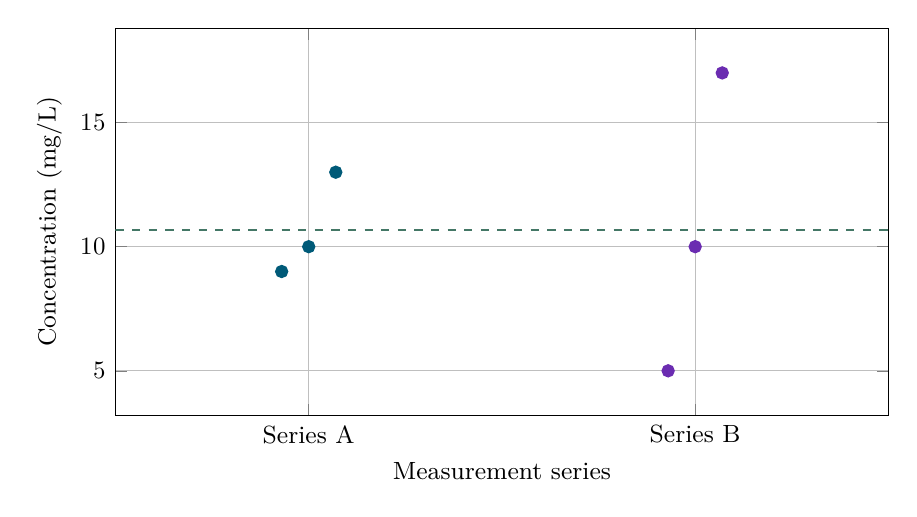
\begin{tikzpicture}
\begin{axis}[width=0.94\linewidth,
height=6.5cm,
scale only axis=false,
grid=major,
tick label style={font=\small},
label style={font=\small},
xlabel={Measurement series},
ylabel={Concentration (mg/L)},
legend style={font=\footnotesize,draw=none,at={(0.5,-0.28)},anchor=north,legend columns=1,text width=0.85\linewidth,align=left},
unbounded coords=jump,
scaled ticks=false,
ymin=3.2,
ymax=18.8,
xmin=0.5,
xmax=2.5,
xtick={1,2},
xticklabels={{Series A},{Series B}}]
\addplot[color=pcd1,thick,only marks,mark=*] coordinates {(0.9299999999999999,9) (1,10) (1.07,13)};
\addplot[color=pcd2,thick,only marks,mark=*] coordinates {(1.93,5) (2,10) (2.07,17)};
\addplot[color=pcd3,thick,dashed,mark=none] coordinates {(0.5,10.667) (2.5,10.667)};

\end{axis}
\end{tikzpicture}
\end{center}


\medskip

A deviation subtracts the observed average from an individual value (\hyperref[material-d6d3849d52167d28da28c231a4bd8d8b9016e465ac60515ad73c34de72c7fca0]{Eq.~\ref*{material-d6d3849d52167d28da28c231a4bd8d8b9016e465ac60515ad73c34de72c7fca0}}). Its sign identifies the side of the centre, and its magnitude gives the distance in the original measurement unit. The signed deviations sum to zero (\hyperref[material-dba7614fdb5c33f7dccca9e1afb51b8e88146bf7d982d85391abedcbd5473095]{Eq.~\ref*{material-dba7614fdb5c33f7dccca9e1afb51b8e88146bf7d982d85391abedcbd5473095}}), an algebraic consequence of centring on the arithmetic mean. Squaring retains information about magnitude when the positive and negative departures balance.


\par\medskip
\noindent\begin{minipage}{\linewidth}
\refstepcounter{equation}\label{material-d6d3849d52167d28da28c231a4bd8d8b9016e465ac60515ad73c34de72c7fca0}
\noindent\textbf{Eq.~\ref*{material-d6d3849d52167d28da28c231a4bd8d8b9016e465ac60515ad73c34de72c7fca0}.} Deviation of an observed value from its sample mean, in the original measurement unit.\par\nopagebreak
\begin{center}\begin{adjustbox}{max width=\linewidth}$\displaystyle d_i=x_i-\bar{x}$\end{adjustbox}\end{center}

\par\noindent\textbf{Symbols}

\par\noindent\textbf{\(d_i\)} Signed deviation of observation i from its sample mean.

\par\noindent\textbf{\(i\)} Observation index, running from 1 to the declared observation count.

\par\noindent\textbf{\(x_i\)} i-th observed value

\par\noindent\textbf{\(\bar{x}\)} sample arithmetic mean

\end{minipage}\par
\medskip

\par\medskip
\noindent\begin{minipage}{\linewidth}
\refstepcounter{equation}\label{material-dba7614fdb5c33f7dccca9e1afb51b8e88146bf7d982d85391abedcbd5473095}
\noindent\textbf{Eq.~\ref*{material-dba7614fdb5c33f7dccca9e1afb51b8e88146bf7d982d85391abedcbd5473095}.} The signed deviations from the arithmetic mean sum to zero.\par\nopagebreak
\begin{center}\begin{adjustbox}{max width=\linewidth}$\displaystyle \sum_{i=1}^n d_i=0$\end{adjustbox}\end{center}

\par\noindent\textbf{Symbols}

\par\noindent\textbf{\(d_i\)} Signed deviation of observation i from its sample mean.

\par\noindent\textbf{\(i\)} Observation index, running from 1 to the declared observation count.

\par\noindent\textbf{\(n\)} number of observations in the sample

\par\noindent\textbf{\(\sum\)} Sum over the indexed observations.

\end{minipage}\par
\medskip

The sum of squared deviations in \hyperref[material-c3ceac2c4030e5934b7a224623ea5baaac34bae590cdfea954152fa71183a73d]{Eq.~\ref*{material-c3ceac2c4030e5934b7a224623ea5baaac34bae590cdfea954152fa71183a73d}} therefore describes aggregate departure. Dividing it by the number of observations gives the empirical mean squared deviation (\hyperref[material-b4f4eb7a9a55b3b1fc2b4bf7f1b33388a05affebba27687a3c2cb3dffb92ce28]{Eq.~\ref*{material-b4f4eb7a9a55b3b1fc2b4bf7f1b33388a05affebba27687a3c2cb3dffb92ce28}}), a descriptive summary of this finite data set. Squaring the original measurement unit is part of its meaning. Taking a square root later returns a spread summary to the original scale.


\par\medskip
\noindent\begin{minipage}{\linewidth}
\refstepcounter{equation}\label{material-c3ceac2c4030e5934b7a224623ea5baaac34bae590cdfea954152fa71183a73d}
\noindent\textbf{Eq.~\ref*{material-c3ceac2c4030e5934b7a224623ea5baaac34bae590cdfea954152fa71183a73d}.} Sum of squared deviations from the observed mean, with squared units.\par\nopagebreak
\begin{center}\begin{adjustbox}{max width=\linewidth}$\displaystyle \begin{gathered}d_i^2=(x_i-\bar{x})^2\\SS=\sum_{i=1}^{n}d_i^2\end{gathered}$\end{adjustbox}\end{center}

\par\noindent\textbf{Symbols}

\par\noindent\textbf{Square each deviation} x\ensuremath{{}_i}: observation i; i: index; \ensuremath{\bar{x}}: sample mean; d\ensuremath{{}_i}: their signed difference. Superscript 2 denotes squaring.

\par\noindent\textbf{SS: Sum of Squares} n: observation count; \ensuremath{\Sigma}: sum from 1 to n. SS adds the squared deviations. Squaring mg/L produces the unit (mg/L)\ensuremath{{}^2}.

\end{minipage}\par
\medskip

\par\medskip
\noindent\begin{minipage}{\linewidth}
\refstepcounter{equation}\label{material-b4f4eb7a9a55b3b1fc2b4bf7f1b33388a05affebba27687a3c2cb3dffb92ce28}
\noindent\textbf{Eq.~\ref*{material-b4f4eb7a9a55b3b1fc2b4bf7f1b33388a05affebba27687a3c2cb3dffb92ce28}.} Empirical mean squared deviation: squared departures averaged over the observed data.\par\nopagebreak
\begin{center}\begin{adjustbox}{max width=\linewidth}$\displaystyle \mathrm{MSD}=\frac{SS}{n}=\frac{\sum_{i=1}^{n}(x_i-\bar{x})^2}{n}$\end{adjustbox}\end{center}

\par\noindent\textbf{Symbols}

\par\noindent\textbf{Mean squared deviation} MSD: mean squared deviation; SS: sum of squared deviations. x\ensuremath{{}_i}: observation i; i: index; \ensuremath{\bar{x}}: sample mean; n: count; \ensuremath{\Sigma}: sum from 1 to n.

\par\noindent\textbf{Squared unit, not absolute distance} The deviations are squared before averaging, so MSD has unit (mg/L)\ensuremath{{}^2}. Division by a count does not change that unit. MSD is not mean absolute distance.

\end{minipage}\par
\medskip

\clearpage
\section{A finite-data description and a population estimate answer different questions}
Describing the recorded values and estimating variation in a generating population require different reference objects. The empirical quantity in \hyperref[material-d1cc6ed43024da06aed33913a0a3a1e4f539519f26a7cbac581b5db42558f439]{Eq.~\ref*{material-d1cc6ed43024da06aed33913a0a3a1e4f539519f26a7cbac581b5db42558f439}} summarizes the fixed observations. The population quantity in \hyperref[material-8771550c15d10b63af18bf44b8c593566d25787e70ff36df713ef21dd1c66393]{Eq.~\ref*{material-8771550c15d10b63af18bf44b8c593566d25787e70ff36df713ef21dd1c66393}} describes variation under the probability model. To study an estimator, we imagine repeatedly drawing new samples from that model and recalculating the statistic each time.


\par\medskip
\noindent\begin{minipage}{\linewidth}
\refstepcounter{equation}\label{material-d1cc6ed43024da06aed33913a0a3a1e4f539519f26a7cbac581b5db42558f439}
\noindent\textbf{Eq.~\ref*{material-d1cc6ed43024da06aed33913a0a3a1e4f539519f26a7cbac581b5db42558f439}.} Empirical squared-deviation summary of a fixed observed sample.\par\nopagebreak
\begin{center}\begin{adjustbox}{max width=\linewidth}$\displaystyle \mathrm{MSD}_n=\frac1n{\textstyle\sum_{i=1}^n}(x_i-\bar x)^2$\end{adjustbox}\end{center}

\par\noindent\textbf{Symbols}

\par\noindent\textbf{\(\mathrm{MSD}_n\)} Mean squared deviation about the fitted sample mean, with divisor n; a statistic across repeated samples.

\par\noindent\textbf{\(i\)} Observation index, running from 1 to the declared observation count.

\par\noindent\textbf{\(n\)} number of observations in the sample

\par\noindent\textbf{\(x_i\)} i-th observed value

\par\noindent\textbf{\(\bar{x}\)} sample arithmetic mean

\par\noindent\textbf{\(\sum\)} Sum over the indexed observations.

\end{minipage}\par
\medskip

\par\medskip
\noindent\begin{minipage}{\linewidth}
\refstepcounter{equation}\label{material-8771550c15d10b63af18bf44b8c593566d25787e70ff36df713ef21dd1c66393}
\noindent\textbf{Eq.~\ref*{material-8771550c15d10b63af18bf44b8c593566d25787e70ff36df713ef21dd1c66393}.} Population variance as an expectation under the specified probability model.\par\nopagebreak
\begin{center}\begin{adjustbox}{max width=\linewidth}$\displaystyle \begin{aligned}\mu&=\operatorname{E}[X]\\\operatorname{Var}(X)&=\operatorname{E}[(X-\operatorname{E}[X])^2]\\&=\operatorname{E}[(X-\mu)^2]=\sigma^2\end{aligned}$\end{adjustbox}\end{center}

\par\noindent\textbf{Symbols}

\par\noindent\textbf{\(\operatorname{E}\)} Expectation, the probability-weighted average of a random quantity under repeated sampling.

\par\noindent\textbf{\(\operatorname{Var}\)} Variance: expected squared deviation of a random quantity from its expectation.

\par\noindent\textbf{\(X\)} One random observation from the population, before a specific value is observed.

\par\noindent\textbf{\(\mu\)} population mean

\par\noindent\textbf{\(\sigma^2\)} Population variance, the expected squared deviation from the population mean.

\end{minipage}\par
\medskip

Expectation rules express the average behaviour over those repeated samples. Fixed-factor and linearity rules appear in \hyperref[material-400ea9141ff850402a14f4a3a53b8d5d6cec0a0fa276143399cd5192e74bbcb7]{Eq.~\ref*{material-400ea9141ff850402a14f4a3a53b8d5d6cec0a0fa276143399cd5192e74bbcb7}} and \hyperref[material-1ab814606c026da238abfd3e1ac10c3c95c40b28a62d0bd86049e530e78e8f68]{Eq.~\ref*{material-1ab814606c026da238abfd3e1ac10c3c95c40b28a62d0bd86049e530e78e8f68}}. Variance rules additionally account for dependence: \hyperref[material-4c9a4b84abd134a62ca883706031fdf3bc17fac540d54f8ed2a4f76d20b7de8c]{Eq.~\ref*{material-4c9a4b84abd134a62ca883706031fdf3bc17fac540d54f8ed2a4f76d20b7de8c}} handles fixed transformations, and \hyperref[material-8ea69b12628e07d5f5e950b4833946586e13dccaf128878d0c5b0b069d72926d]{Eq.~\ref*{material-8ea69b12628e07d5f5e950b4833946586e13dccaf128878d0c5b0b069d72926d}} retains covariance contributions. Independence is a sufficient condition for the relevant covariance terms to vanish; the assumptions must match the sampling design.


\par\medskip
\noindent\begin{minipage}{\linewidth}
\refstepcounter{equation}\label{material-400ea9141ff850402a14f4a3a53b8d5d6cec0a0fa276143399cd5192e74bbcb7}
\noindent\textbf{Eq.~\ref*{material-400ea9141ff850402a14f4a3a53b8d5d6cec0a0fa276143399cd5192e74bbcb7}.} Expectation rule for fixed terms, with the full authored conventions.\par\nopagebreak
\begin{center}\begin{adjustbox}{max width=\linewidth}$\displaystyle \begin{gathered}\operatorname{E}[c]=c\\\operatorname{E}[aY+b]=a\operatorname{E}[Y]+b\end{gathered}$\end{adjustbox}\end{center}

\par\noindent\textbf{Symbols}

\par\noindent\textbf{\(\operatorname{E}\)} Expectation, the probability-weighted average of a random quantity under repeated sampling.

\par\noindent\textbf{\(Y\)} A random quantity with the moments required by the stated identity.

\par\noindent\textbf{\(a\)} Fixed real scale factor in an affine transformation.

\par\noindent\textbf{\(b\)} Fixed real additive shift in an affine transformation.

\par\noindent\textbf{\(c\)} A scalar placeholder; a fixed constant when pulled outside a sum or expectation.

\end{minipage}\par
\medskip

\par\medskip
\noindent\begin{minipage}{\linewidth}
\refstepcounter{equation}\label{material-1ab814606c026da238abfd3e1ac10c3c95c40b28a62d0bd86049e530e78e8f68}
\noindent\textbf{Eq.~\ref*{material-1ab814606c026da238abfd3e1ac10c3c95c40b28a62d0bd86049e530e78e8f68}.} Linearity of expectation for the authored random quantities.\par\nopagebreak
\begin{center}\begin{adjustbox}{max width=\linewidth}$\displaystyle \begin{gathered}\operatorname{E}[U+V]=\operatorname{E}[U]+\operatorname{E}[V]\\\operatorname{E}[{\textstyle\sum_{i=1}^n}Y_i]={\textstyle\sum_{i=1}^n}\operatorname{E}[Y_i]\end{gathered}$\end{adjustbox}\end{center}

\par\noindent\textbf{Symbols}

\par\noindent\textbf{\(\operatorname{E}\)} Expectation, the probability-weighted average of a random quantity under repeated sampling.

\par\noindent\textbf{\(U\)} An integrable random quantity in an expectation identity.

\par\noindent\textbf{\(V\)} A second integrable random quantity.

\par\noindent\textbf{\(Y_i\)} The indexed random quantity i in a finite sum.

\par\noindent\textbf{\(i\)} Observation index, running from 1 to the declared observation count.

\par\noindent\textbf{\(n\)} number of observations in the sample

\par\noindent\textbf{\(\sum\)} Sum over the indexed observations.

\end{minipage}\par
\medskip

\par\medskip
\noindent\begin{minipage}{\linewidth}
\refstepcounter{equation}\label{material-4c9a4b84abd134a62ca883706031fdf3bc17fac540d54f8ed2a4f76d20b7de8c}
\noindent\textbf{Eq.~\ref*{material-4c9a4b84abd134a62ca883706031fdf3bc17fac540d54f8ed2a4f76d20b7de8c}.} Variance under fixed shifts and scaling.\par\nopagebreak
\begin{center}\begin{adjustbox}{max width=\linewidth}$\displaystyle \begin{gathered}\operatorname{Var}(c)=0\\\operatorname{Var}(aY+b)=a^2\operatorname{Var}(Y)\end{gathered}$\end{adjustbox}\end{center}

\par\noindent\textbf{Symbols}

\par\noindent\textbf{\(\operatorname{Var}\)} Variance: expected squared deviation of a random quantity from its expectation.

\par\noindent\textbf{\(Y\)} A random quantity with the moments required by the stated identity.

\par\noindent\textbf{\(a\)} Fixed real scale factor in an affine transformation.

\par\noindent\textbf{\(b\)} Fixed real additive shift in an affine transformation.

\par\noindent\textbf{\(c\)} A scalar placeholder; a fixed constant when pulled outside a sum or expectation.

\end{minipage}\par
\medskip

\par\medskip
\noindent\begin{minipage}{\linewidth}
\refstepcounter{equation}\label{material-8ea69b12628e07d5f5e950b4833946586e13dccaf128878d0c5b0b069d72926d}
\noindent\textbf{Eq.~\ref*{material-8ea69b12628e07d5f5e950b4833946586e13dccaf128878d0c5b0b069d72926d}.} Variance of combined random quantities, including covariance and its conditions.\par\nopagebreak
\begin{center}\begin{adjustbox}{max width=\linewidth}$\displaystyle \begin{aligned}\operatorname{Var}(U+V)&=\operatorname{Var}(U)+\operatorname{Var}(V)\\&\quad+2\operatorname{Cov}(U,V)\\\operatorname{Cov}(U,V)&=\operatorname{E}[(U-\operatorname{E}[U])\\&\qquad\cdot(V-\operatorname{E}[V])]\end{aligned}$\end{adjustbox}\end{center}

\par\noindent\textbf{Symbols}

\par\noindent\textbf{\(\operatorname{Cov}\)} Covariance of two random quantities; it measures their joint linear variation.

\par\noindent\textbf{\(\operatorname{E}\)} Expectation, the probability-weighted average of a random quantity under repeated sampling.

\par\noindent\textbf{\(U\)} An integrable random quantity in an expectation identity.

\par\noindent\textbf{\(V\)} A second integrable random quantity.

\par\noindent\textbf{\(\operatorname{Var}\)} Variance: expected squared deviation of a random quantity from its expectation.

\end{minipage}\par
\medskip

The random-sample expression in \hyperref[material-c2003691e3a44889f1e5f4d0d7b9db840acf717c20dedad0059b42d53e0f5565]{Eq.~\ref*{material-c2003691e3a44889f1e5f4d0d7b9db840acf717c20dedad0059b42d53e0f5565}} makes the empirical calculation into an estimator. Its target question is stated in \hyperref[material-06eb254d2f64c2602b6475199630cafda1c5aa0f84305cbb205e9ca54e90c820]{Eq.~\ref*{material-06eb254d2f64c2602b6475199630cafda1c5aa0f84305cbb205e9ca54e90c820}}. The repeated-sampling simulation in \hyperref[material-a90f33ba78efcaec86dd2a6111a5278c3097092b9868b2cf3b25d5facbe1beb7]{Fig.~\ref*{material-a90f33ba78efcaec86dd2a6111a5278c3097092b9868b2cf3b25d5facbe1beb7}} illustrates how the resulting estimates vary. Averaging estimates over many simulated samples investigates the estimator's expectation under the chosen model; the spread of those estimates describes a second, sampling-level source of variation.


\par\medskip
\noindent\begin{minipage}{\linewidth}
\refstepcounter{equation}\label{material-c2003691e3a44889f1e5f4d0d7b9db840acf717c20dedad0059b42d53e0f5565}
\noindent\textbf{Eq.~\ref*{material-c2003691e3a44889f1e5f4d0d7b9db840acf717c20dedad0059b42d53e0f5565}.} Mean squared deviation calculated from a random sample and its random sample mean.\par\nopagebreak
\begin{center}\begin{adjustbox}{max width=\linewidth}$\displaystyle \mathrm{MSD}_n=\frac1n{\textstyle\sum_{i=1}^n}(X_i-\bar X)^2$\end{adjustbox}\end{center}

\par\noindent\textbf{Symbols}

\par\noindent\textbf{\(\mathrm{MSD}_n\)} Mean squared deviation about the fitted sample mean, with divisor n; a statistic across repeated samples.

\par\noindent\textbf{\(X_i\)} Random observation i before its value x\_i is observed.

\par\noindent\textbf{\(\bar X\)} Random sample mean across repeated samples, as distinct from an observed sample mean \ensuremath{\bar{x}}.

\par\noindent\textbf{\(i\)} Observation index, running from 1 to the declared observation count.

\par\noindent\textbf{\(n\)} number of observations in the sample

\par\noindent\textbf{\(\sum\)} Sum over the indexed observations.

\end{minipage}\par
\medskip

\par\medskip
\noindent\begin{minipage}{\linewidth}
\refstepcounter{equation}\label{material-06eb254d2f64c2602b6475199630cafda1c5aa0f84305cbb205e9ca54e90c820}
\noindent\textbf{Eq.~\ref*{material-06eb254d2f64c2602b6475199630cafda1c5aa0f84305cbb205e9ca54e90c820}.} Expectation question connecting the random squared-deviation summary with population variance.\par\nopagebreak
\begin{center}\begin{adjustbox}{max width=\linewidth}$\displaystyle \operatorname{E}[\mathrm{MSD}_n]\;\overset{?}{=}\;\sigma^2$\end{adjustbox}\end{center}

\par\noindent\textbf{Symbols}

\par\noindent\textbf{\(\operatorname{E}\)} Expectation, the probability-weighted average of a random quantity under repeated sampling.

\par\noindent\textbf{\(\mathrm{MSD}_n\)} Mean squared deviation about the fitted sample mean, with divisor n; a statistic across repeated samples.

\par\noindent\textbf{\(\sigma^2\)} Population variance, the expected squared deviation from the population mean.

\end{minipage}\par
\medskip

\par\medskip
\Needspace{10cm}
\refstepcounter{figure}\label{material-a90f33ba78efcaec86dd2a6111a5278c3097092b9868b2cf3b25d5facbe1beb7}
\noindent\textbf{Fig.~\ref*{material-a90f33ba78efcaec86dd2a6111a5278c3097092b9868b2cf3b25d5facbe1beb7}.} Repeated-sampling simulation of the variance calculation under the authored model and parameters.\par\nopagebreak
\begin{center}
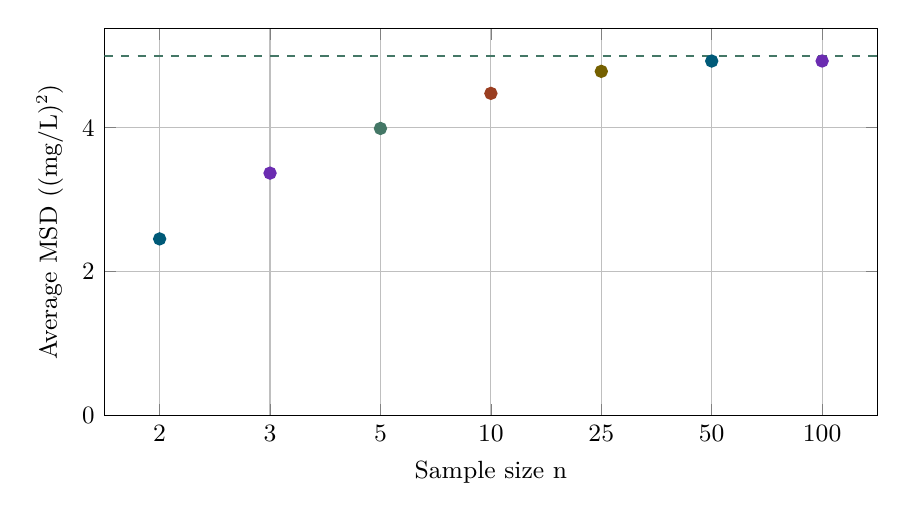
\begin{tikzpicture}
\begin{axis}[width=0.94\linewidth,
height=6.5cm,
scale only axis=false,
grid=major,
tick label style={font=\small},
label style={font=\small},
xlabel={Sample size n},
ylabel={Average MSD ((mg/L)\ensuremath{{}^2})},
legend style={font=\footnotesize,draw=none,at={(0.5,-0.28)},anchor=north,legend columns=1,text width=0.85\linewidth,align=left},
unbounded coords=jump,
scaled ticks=false,
ymin=0,
ymax=5.3818541,
xmin=0.5,
xmax=7.5,
xtick={1,2,3,4,5,6,7},
xticklabels={{2},{3},{5},{10},{25},{50},{100}}]
\addplot[color=pcd1,thick,only marks,mark=*] coordinates {(1,2.454306)};
\addplot[color=pcd2,thick,only marks,mark=*] coordinates {(2,3.368247)};
\addplot[color=pcd3,thick,only marks,mark=*] coordinates {(3,3.989123)};
\addplot[color=pcd4,thick,only marks,mark=*] coordinates {(4,4.476612)};
\addplot[color=pcd5,thick,only marks,mark=*] coordinates {(5,4.782485)};
\addplot[color=pcd1,thick,only marks,mark=*] coordinates {(6,4.925768)};
\addplot[color=pcd2,thick,only marks,mark=*] coordinates {(7,4.926258)};
\addplot[color=pcd3,thick,dashed,mark=none] coordinates {(0.5,5) (7.5,5)};

\end{axis}
\end{tikzpicture}
\end{center}


\medskip

\clearpage
\section{Estimating the centre changes the variance estimator's expectation}
The sample mean is calculated from the same observations whose departures are being squared. This shared origin matters: a fitted centre follows the sample and reduces its aggregate squared departure relative to using the population centre. The algebra in \hyperref[material-c95b90bfca60127e39921090acdf828d49a4c6b004cd779aa35ee13d6f906e15]{Eq.~\ref*{material-c95b90bfca60127e39921090acdf828d49a4c6b004cd779aa35ee13d6f906e15}} separates those contributions before any expectation is taken.


\par\medskip
\Needspace{8\baselineskip}
\refstepcounter{equation}\label{material-c95b90bfca60127e39921090acdf828d49a4c6b004cd779aa35ee13d6f906e15}
\noindent\textbf{Eq.~\ref*{material-c95b90bfca60127e39921090acdf828d49a4c6b004cd779aa35ee13d6f906e15}.} Stepwise squared-deviation decomposition, retaining the authored operations, explanations and symbol legend.\par\nopagebreak
\paragraph{Find the source of the MSD shortfall}
\begin{center}\begin{adjustbox}{max width=\linewidth}$\displaystyle X_i-\bar X=(X_i-\mu)-(\bar X-\mu)$\end{adjustbox}\end{center}
\noindent\textbf{Square, sum and collect the centered terms} (Mathematical implication)\par
Expand each centered difference, distribute the finite sum, and use \ensuremath{\Sigma}(a\_i\ensuremath{-}c) = n(\ensuremath{\bar{a}}\ensuremath{-}c). The two cross-term contributions combine with the last squared shift to leave one negative squared shift. The fitted mean removes a nonnegative term. This is an exact algebraic identity for each realization, not an expectation or an unbiasedness claim.
\begin{center}\begin{adjustbox}{max width=\linewidth}$\displaystyle \begin{aligned}\frac1n\sum_i(a_i-\bar a)^2&=\frac1n\sum_i(a_i-c)^2\\&\quad-(\bar a-c)^2\end{aligned}$\end{adjustbox}\end{center}

Centering at the fitted arithmetic mean removes a nonnegative squared shift. The result is an exact identity, not an average statement. Open the full algebra detail for each expansion and summation operation. The population mean is ordinarily unknown; this identity explains the estimator, rather than giving a formula that requires knowing \ensuremath{\mu}.
\begin{center}\begin{adjustbox}{max width=\linewidth}$\displaystyle \boxed{\begin{aligned}\mathrm{MSD}_n&=\frac1n\sum_{i=1}^n(X_i-\mu)^2\\&\quad-(\bar X-\mu)^2\end{aligned}}$\end{adjustbox}\end{center}

\par\textbf{Arithmetic mean of the same n values} n is a positive integer, \ensuremath{\bar{a}} = (1/n)\ensuremath{\Sigma}a\_i, and c is fixed with respect to the index. The identity holds deterministically for every finite realization.
\begin{center}\begin{adjustbox}{max width=\linewidth}$\displaystyle \boxed{\begin{aligned}\mathrm{MSD}_n&=\frac1n\sum_{i=1}^n(X_i-\mu)^2\\&\quad-(\bar X-\mu)^2\end{aligned}}$\end{adjustbox}\end{center}

\paragraph{Symbols}
\par\noindent\textbf{\(\mathrm{MSD}_n\)} Mean squared deviation about the fitted sample mean, with divisor n; a statistic across repeated samples.
\par\noindent\textbf{\(X_i\)} Random observation i before its value x\_i is observed.
\par\noindent\textbf{\(\bar X\)} Random sample mean across repeated samples, as distinct from an observed sample mean \ensuremath{\bar{x}}.
\par\noindent\textbf{\(i\)} Observation index, running from 1 to the declared observation count.
\par\noindent\textbf{\(n\)} number of observations in the sample
\par\noindent\textbf{\(\sum\)} Sum over the indexed observations.
\par\noindent\textbf{\(\mu\)} population mean
\subsubsection*{Full algebra: why fitting the mean removes a squared shift}
\paragraph{Full algebra: why fitting the mean removes a squared shift}
\begin{center}\begin{adjustbox}{max width=\linewidth}$\displaystyle X_i-\bar X=(X_i-\mu)-(\bar X-\mu)$\end{adjustbox}\end{center}
\noindent\textbf{Square the centered difference and expand} (Mathematical implication)\par
Multiplying a+b by itself gives a\ensuremath{{}^2}, the two equal cross-products ab, and b\ensuremath{{}^2}. Squaring both sides of an equality is a valid implication, not generally a reversible operation without sign information.
\begin{center}\begin{adjustbox}{max width=\linewidth}$\displaystyle (a+b)^2=a^2+2ab+b^2$\end{adjustbox}\end{center}

Use a = X\ensuremath{{}_i}\ensuremath{-}\ensuremath{\mu} and b = \ensuremath{-}(\ensuremath{\bar{X}}\ensuremath{-}\ensuremath{\mu}) in the binomial identity. Squaring an equality gives a consequence; we do not claim to recover all signs by reversing this step.
\begin{center}\begin{adjustbox}{max width=\linewidth}$\displaystyle \begin{aligned}(X_i-\bar X)^2&=(X_i-\mu)^2\\&\quad-2(X_i-\mu)(\bar X-\mu)\\&\quad+(\bar X-\mu)^2\end{aligned}$\end{adjustbox}\end{center}


\begin{center}\begin{adjustbox}{max width=\linewidth}$\displaystyle \begin{aligned}(X_i-\bar X)^2&=(X_i-\mu)^2\\&\quad-2(X_i-\mu)(\bar X-\mu)\\&\quad+(\bar X-\mu)^2\end{aligned}$\end{adjustbox}\end{center}

\paragraph{Symbols}
\par\noindent\textbf{\(X_i\)} Random observation i before its value x\_i is observed.
\par\noindent\textbf{\(\bar X\)} Random sample mean across repeated samples, as distinct from an observed sample mean \ensuremath{\bar{x}}.
\par\noindent\textbf{\(\mu\)} population mean
\paragraph{Full algebra: why fitting the mean removes a squared shift}
\begin{center}\begin{adjustbox}{max width=\linewidth}$\displaystyle \begin{aligned}(X_i-\bar X)^2&=(X_i-\mu)^2\\&\quad-2(X_i-\mu)(\bar X-\mu)\\&\quad+(\bar X-\mu)^2\end{aligned}$\end{adjustbox}\end{center}
\noindent\textbf{Sum, divide by n and factor index-independent terms} (Mathematical implication)\par
Use linearity for each of the three summands and move the index-independent coefficient c outside the middle sum. The last sum is not simplified yet.
\begin{center}\begin{adjustbox}{max width=\linewidth}$\displaystyle \begin{gathered}\sum_{i=1}^n(a_i+cb_i+q)\\=\sum_{i=1}^n a_i+c\sum_{i=1}^n b_i\\+\sum_{i=1}^n q\end{gathered}$\end{adjustbox}\end{center}

Distribute the finite sum over the three terms, then divide by the positive n. The same \ensuremath{\bar{X}}\ensuremath{-}\ensuremath{\mu} occurs at every index, so it factors out of the cross term. Its squared last term is added n times; the divisor n cancels that count. This is deterministic within each realization.
\begin{center}\begin{adjustbox}{max width=\linewidth}$\displaystyle \begin{aligned}\frac1n\sum_i(X_i-\bar X)^2&=\frac1n\sum_i(X_i-\mu)^2\\&\quad-\frac2n(\bar X-\mu)\sum_i(X_i-\mu)\\&\quad+(\bar X-\mu)^2\end{aligned}$\end{adjustbox}\end{center}

\par\textbf{Constant with respect to the index} c has the same value for every index i within the sum; n is a positive integer.
\begin{center}\begin{adjustbox}{max width=\linewidth}$\displaystyle \begin{aligned}\frac1n\sum_i(X_i-\bar X)^2&=\frac1n\sum_i(X_i-\mu)^2\\&\quad-\frac2n(\bar X-\mu)\sum_i(X_i-\mu)\\&\quad+(\bar X-\mu)^2\end{aligned}$\end{adjustbox}\end{center}

\paragraph{Symbols}
\par\noindent\textbf{\(X_i\)} Random observation i before its value x\_i is observed.
\par\noindent\textbf{\(\bar X\)} Random sample mean across repeated samples, as distinct from an observed sample mean \ensuremath{\bar{x}}.
\par\noindent\textbf{\(i\)} Observation index, running from 1 to the declared observation count.
\par\noindent\textbf{\(n\)} number of observations in the sample
\par\noindent\textbf{\(\sum\)} Sum over the indexed observations.
\par\noindent\textbf{\(\mu\)} population mean
\paragraph{Full algebra: why fitting the mean removes a squared shift}
\begin{center}\begin{adjustbox}{max width=\linewidth}$\displaystyle \begin{aligned}\frac1n\sum_i(X_i-\bar X)^2&=\frac1n\sum_i(X_i-\mu)^2\\&\quad-\frac2n(\bar X-\mu)\sum_i(X_i-\mu)\\&\quad+(\bar X-\mu)^2\end{aligned}$\end{adjustbox}\end{center}
\noindent\textbf{Insert the sum of population-centered distances} (Equivalent transformation)\par
Split the finite sum over subtraction, count c exactly n times, and substitute \ensuremath{\Sigma}a\_i = n \ensuremath{\bar{a}}. This needs the arithmetic mean of those same values and does not require probability assumptions.
\begin{center}\begin{adjustbox}{max width=\linewidth}$\displaystyle \sum_{i=1}^n(a_i-c)=n(\bar a-c)$\end{adjustbox}\end{center}

\ensuremath{\Sigma}(X\ensuremath{{}_i}\ensuremath{-}\ensuremath{\mu}) = \ensuremath{\Sigma}X\ensuremath{{}_i}\ensuremath{-}n\ensuremath{\mu} = n(\ensuremath{\bar{X}}\ensuremath{-}\ensuremath{\mu}), because \ensuremath{\bar{X}} is the mean of these same observations. Substitute that sum into the cross term: \ensuremath{-}(2/n)(\ensuremath{\bar{X}}\ensuremath{-}\ensuremath{\mu})n(\ensuremath{\bar{X}}\ensuremath{-}\ensuremath{\mu}) = \ensuremath{-}2(\ensuremath{\bar{X}}\ensuremath{-}\ensuremath{\mu})\ensuremath{{}^2}.
\begin{center}\begin{adjustbox}{max width=\linewidth}$\displaystyle \begin{aligned}\frac1n\sum_i(X_i-\bar X)^2&=\frac1n\sum_i(X_i-\mu)^2\\&\quad-2(\bar X-\mu)^2+(\bar X-\mu)^2\end{aligned}$\end{adjustbox}\end{center}

\par\textbf{Arithmetic mean of the same n values} n is a positive integer, \ensuremath{\bar{a}} = (1/n)\ensuremath{\Sigma}a\_i, and c is fixed with respect to the index. The identity holds deterministically for every finite realization.
\begin{center}\begin{adjustbox}{max width=\linewidth}$\displaystyle \begin{aligned}\frac1n\sum_i(X_i-\bar X)^2&=\frac1n\sum_i(X_i-\mu)^2\\&\quad-2(\bar X-\mu)^2+(\bar X-\mu)^2\end{aligned}$\end{adjustbox}\end{center}

\paragraph{Symbols}
\par\noindent\textbf{\(X_i\)} Random observation i before its value x\_i is observed.
\par\noindent\textbf{\(\bar X\)} Random sample mean across repeated samples, as distinct from an observed sample mean \ensuremath{\bar{x}}.
\par\noindent\textbf{\(i\)} Observation index, running from 1 to the declared observation count.
\par\noindent\textbf{\(n\)} number of observations in the sample
\par\noindent\textbf{\(\sum\)} Sum over the indexed observations.
\par\noindent\textbf{\(\mu\)} population mean
\paragraph{Full algebra: why fitting the mean removes a squared shift}
\begin{center}\begin{adjustbox}{max width=\linewidth}$\displaystyle \begin{aligned}\frac1n\sum_i(X_i-\bar X)^2&=\frac1n\sum_i(X_i-\mu)^2\\&\quad-2(\bar X-\mu)^2+(\bar X-\mu)^2\end{aligned}$\end{adjustbox}\end{center}
\noindent\textbf{Combine the squared shifts and identify the MSD} (Equivalent transformation)\par
Expand each centered difference, distribute the finite sum, and use \ensuremath{\Sigma}(a\_i\ensuremath{-}c) = n(\ensuremath{\bar{a}}\ensuremath{-}c). The two cross-term contributions combine with the last squared shift to leave one negative squared shift. The fitted mean removes a nonnegative term. This is an exact algebraic identity for each realization, not an expectation or an unbiasedness claim.
\begin{center}\begin{adjustbox}{max width=\linewidth}$\displaystyle \begin{aligned}\frac1n\sum_i(a_i-\bar a)^2&=\frac1n\sum_i(a_i-c)^2\\&\quad-(\bar a-c)^2\end{aligned}$\end{adjustbox}\end{center}

The coefficients of the shared squared shift are \ensuremath{-}2 and +1, leaving \ensuremath{-}1. The left side is the defining MSD about the fitted sample mean. The result is exact for every sample. It does not by itself prove the estimator's average bias.
\begin{center}\begin{adjustbox}{max width=\linewidth}$\displaystyle \boxed{\begin{aligned}\mathrm{MSD}_n&=\frac1n\sum_{i=1}^n(X_i-\mu)^2\\&\quad-(\bar X-\mu)^2\end{aligned}}$\end{adjustbox}\end{center}

\par\textbf{Arithmetic mean of the same n values} n is a positive integer, \ensuremath{\bar{a}} = (1/n)\ensuremath{\Sigma}a\_i, and c is fixed with respect to the index. The identity holds deterministically for every finite realization.
\begin{center}\begin{adjustbox}{max width=\linewidth}$\displaystyle \boxed{\begin{aligned}\mathrm{MSD}_n&=\frac1n\sum_{i=1}^n(X_i-\mu)^2\\&\quad-(\bar X-\mu)^2\end{aligned}}$\end{adjustbox}\end{center}

\paragraph{Symbols}
\par\noindent\textbf{\(\mathrm{MSD}_n\)} Mean squared deviation about the fitted sample mean, with divisor n; a statistic across repeated samples.
\par\noindent\textbf{\(X_i\)} Random observation i before its value x\_i is observed.
\par\noindent\textbf{\(\bar X\)} Random sample mean across repeated samples, as distinct from an observed sample mean \ensuremath{\bar{x}}.
\par\noindent\textbf{\(i\)} Observation index, running from 1 to the declared observation count.
\par\noindent\textbf{\(n\)} number of observations in the sample
\par\noindent\textbf{\(\sum\)} Sum over the indexed observations.
\par\noindent\textbf{\(\mu\)} population mean
\medskip

Applying the stated sampling assumptions gives the expectation calculation in \hyperref[material-3fc344916e0dc7797c94846b33887833595d45f58abcc8e927bd3872016e474d]{Eq.~\ref*{material-3fc344916e0dc7797c94846b33887833595d45f58abcc8e927bd3872016e474d}}. The variance of the sample mean (\hyperref[material-2306468ba7224c8f5f3277dae3ab18b9df6720a7453d963e9da4fac52f2930cc]{Eq.~\ref*{material-2306468ba7224c8f5f3277dae3ab18b9df6720a7453d963e9da4fac52f2930cc}}) supplies the term that accounts for estimating the centre. For independent observations with a common finite variance, dividing the squared-deviation sum by the sample size yields an expectation reduced by the factor shown in \hyperref[material-b81ef95597ed67a6eba33a1ea10bbb4bf86863f91802638951dc9bd7a7c0906e]{Eq.~\ref*{material-b81ef95597ed67a6eba33a1ea10bbb4bf86863f91802638951dc9bd7a7c0906e}}. This identifies the estimator's average relationship to its target.


\par\medskip
\Needspace{8\baselineskip}
\refstepcounter{equation}\label{material-3fc344916e0dc7797c94846b33887833595d45f58abcc8e927bd3872016e474d}
\noindent\textbf{Eq.~\ref*{material-3fc344916e0dc7797c94846b33887833595d45f58abcc8e927bd3872016e474d}.} Expectation of the decomposition under the authored sampling assumptions.\par\nopagebreak
\paragraph{Average the MSD identity and recognize variance}
\begin{center}\begin{adjustbox}{max width=\linewidth}$\displaystyle \begin{aligned}\operatorname{E}[\mathrm{MSD}_n]&=\frac1n\sum_i\operatorname{E}[(X_i-\mu)^2]\\&\quad-\operatorname{E}[(\bar X-\mu)^2]\end{aligned}$\end{adjustbox}\end{center}
\noindent\textbf{Recognize expected centered squares as variances} (Requires statistical assumptions)\par
For a random variable with finite second moment, variance is the expected squared distance from its expectation.
\begin{center}\begin{adjustbox}{max width=\linewidth}$\displaystyle \operatorname{Var}(Y)=\operatorname{E}[(Y-\operatorname{E}[Y])^2]$\end{adjustbox}\end{center}

Linearity gives the displayed expectation of the finite squared-distance average; it needs no independence. Each population-centered squared observation has expectation \ensuremath{\sigma}\ensuremath{{}^2}. The sample mean has expectation \ensuremath{\mu} under the common-mean condition, so its expected squared shift is Var(\ensuremath{\bar{X}}). The arithmetic average of n copies of \ensuremath{\sigma}\ensuremath{{}^2} is \ensuremath{\sigma}\ensuremath{{}^2}. The complete sample-mean argument is available with the next result.
\begin{center}\begin{adjustbox}{max width=\linewidth}$\displaystyle \begin{gathered}\operatorname{E}[(X_i-\mu)^2]=\sigma^2\\\operatorname{E}[(\bar X-\mu)^2]=\operatorname{Var}(\bar X)\end{gathered}$\end{adjustbox}\end{center}

\par\textbf{Common mean and finite variance; fixed n \ensuremath{\ge} 1} For each i = 1, \ensuremath{\ldots}, n, E[X\_i] = \ensuremath{\mu} and Var(X\_i) = \ensuremath{\sigma}\ensuremath{{}^2} < \ensuremath{\infty}. The positive integer n is fixed. Identical distribution is sufficient but equality of these moments is all that is needed here.
\par\textbf{Finite second moment} Y has a finite second moment, so its expectation and variance exist.
\begin{center}\begin{adjustbox}{max width=\linewidth}$\displaystyle \operatorname{E}[\mathrm{MSD}_n]=\sigma^2-\operatorname{Var}(\bar X)$\end{adjustbox}\end{center}

\paragraph{Symbols}
\par\noindent\textbf{\(\operatorname{E}\)} Expectation, the probability-weighted average of a random quantity under repeated sampling.
\par\noindent\textbf{\(\mathrm{MSD}_n\)} Mean squared deviation about the fitted sample mean, with divisor n; a statistic across repeated samples.
\par\noindent\textbf{\(\operatorname{Var}\)} Variance: expected squared deviation of a random quantity from its expectation.
\par\noindent\textbf{\(X_i\)} Random observation i before its value x\_i is observed.
\par\noindent\textbf{\(\bar X\)} Random sample mean across repeated samples, as distinct from an observed sample mean \ensuremath{\bar{x}}.
\par\noindent\textbf{\(i\)} Observation index, running from 1 to the declared observation count.
\par\noindent\textbf{\(n\)} number of observations in the sample
\par\noindent\textbf{\(\sum\)} Sum over the indexed observations.
\par\noindent\textbf{\(\mu\)} population mean
\par\noindent\textbf{\(\sigma^2\)} Population variance, the expected squared deviation from the population mean.
\medskip

\par\medskip
\noindent\begin{minipage}{\linewidth}
\refstepcounter{equation}\label{material-2306468ba7224c8f5f3277dae3ab18b9df6720a7453d963e9da4fac52f2930cc}
\noindent\textbf{Eq.~\ref*{material-2306468ba7224c8f5f3277dae3ab18b9df6720a7453d963e9da4fac52f2930cc}.} Variance of the sample mean under the stated common-variance sampling model.\par\nopagebreak
\begin{center}\begin{adjustbox}{max width=\linewidth}$\displaystyle \boxed{\operatorname{Var}(\bar X)=\frac{\sigma^2}{n}}$\end{adjustbox}\end{center}

\par\noindent\textbf{Symbols}

\par\noindent\textbf{\(\operatorname{Var}\)} Variance: expected squared deviation of a random quantity from its expectation.

\par\noindent\textbf{\(\bar X\)} Random sample mean across repeated samples, as distinct from an observed sample mean \ensuremath{\bar{x}}.

\par\noindent\textbf{\(n\)} number of observations in the sample

\par\noindent\textbf{\(\sigma^2\)} Population variance, the expected squared deviation from the population mean.

\end{minipage}\par
\medskip

\par\medskip
\Needspace{8\baselineskip}
\refstepcounter{equation}\label{material-b81ef95597ed67a6eba33a1ea10bbb4bf86863f91802638951dc9bd7a7c0906e}
\noindent\textbf{Eq.~\ref*{material-b81ef95597ed67a6eba33a1ea10bbb4bf86863f91802638951dc9bd7a7c0906e}.} Expectation factor for the squared-deviation estimator divided by sample size.\par\nopagebreak
\paragraph{From the fitted-mean identity to unbiased variance}
\begin{center}\begin{adjustbox}{max width=\linewidth}$\displaystyle \operatorname{E}[\mathrm{MSD}_n]=\sigma^2-\frac{\sigma^2}{n}$\end{adjustbox}\end{center}
\noindent\textbf{Factor out the population variance} (Equivalent transformation)\par
Write a as na/n, subtract a/n and factor out a. The result holds for every real a and positive integer n. This is algebra, not an additional statistical assumption.
\begin{center}\begin{adjustbox}{max width=\linewidth}$\displaystyle a-\frac an=\frac{n-1}{n}a$\end{adjustbox}\end{center}

In the general factorization use a = \ensuremath{\sigma}\ensuremath{{}^2}.
The fraction left after subtraction is (n\ensuremath{-}1)/n, strictly less than one for n > 1. Thus the MSD is biased downward when \ensuremath{\sigma}\ensuremath{{}^2} > 0.
A particular realized MSD may lie above or below \ensuremath{\sigma}\ensuremath{{}^2}. Bias is the repeated-sampling expectation, not the direction of every individual error.
\begin{center}\begin{adjustbox}{max width=\linewidth}$\displaystyle \operatorname{E}[\mathrm{MSD}_n]=\frac{n-1}{n}\sigma^2$\end{adjustbox}\end{center}

\par\textbf{Finite observation count} n is a positive integer; all indexed equalities hold for i = 1, \ensuremath{\ldots}, n.
\begin{center}\begin{adjustbox}{max width=\linewidth}$\displaystyle \operatorname{E}[\mathrm{MSD}_n]=\frac{n-1}{n}\sigma^2$\end{adjustbox}\end{center}

\paragraph{Symbols}
\par\noindent\textbf{\(\operatorname{E}\)} Expectation, the probability-weighted average of a random quantity under repeated sampling.
\par\noindent\textbf{\(\mathrm{MSD}_n\)} Mean squared deviation about the fitted sample mean, with divisor n; a statistic across repeated samples.
\par\noindent\textbf{\(n\)} number of observations in the sample
\par\noindent\textbf{\(\sigma^2\)} Population variance, the expected squared deviation from the population mean.
\medskip

Bessel's correction compensates for that factor (\hyperref[material-3a721ace44a7a90b9c00bd891e70a88bac9e4dbe6ec7bc9efd61a352241b4b11]{Eq.~\ref*{material-3a721ace44a7a90b9c00bd891e70a88bac9e4dbe6ec7bc9efd61a352241b4b11}}). For at least two observations under the stated common-variance, uncorrelated sampling conditions, the practical formula in \hyperref[material-b35860b413f4a3c576a46862c353d1453267a82e3f62bbfec1ad04fdbff55b99]{Eq.~\ref*{material-b35860b413f4a3c576a46862c353d1453267a82e3f62bbfec1ad04fdbff55b99}} is unbiased for population variance. The simulation in \hyperref[material-e9704c5f7a432f059f21ba0d47de209341464e13c274da8f1e7f2ca618c1234c]{Fig.~\ref*{material-e9704c5f7a432f059f21ba0d47de209341464e13c274da8f1e7f2ca618c1234c}} compares this expectation behaviour across repeated samples. Unbiasedness describes an average over sampling; a particular sample still supplies an estimate with its own sampling variation.


\par\medskip
\Needspace{8\baselineskip}
\refstepcounter{equation}\label{material-3a721ace44a7a90b9c00bd891e70a88bac9e4dbe6ec7bc9efd61a352241b4b11}
\noindent\textbf{Eq.~\ref*{material-3a721ace44a7a90b9c00bd891e70a88bac9e4dbe6ec7bc9efd61a352241b4b11}.} Bessel correction derived from the estimator's expectation factor.\par\nopagebreak
\paragraph{Bessel's correction}
\begin{center}\begin{adjustbox}{max width=\linewidth}$\displaystyle \operatorname{E}[\mathrm{MSD}_n]=\frac{n-1}{n}\sigma^2$\end{adjustbox}\end{center}
\noindent\textbf{Multiply by the reciprocal bias factor, for n > 1} (Requires statistical assumptions)\par
A constant fixed across repeated samples multiplies the expectation. A random offset such as Δ must not itself be pulled outside E; the fixed count n may be.
\begin{center}\begin{adjustbox}{max width=\linewidth}$\displaystyle \operatorname{E}[cY]=c\operatorname{E}[Y]$\end{adjustbox}\end{center}

Define the random statistic S\ensuremath{{}^2} by multiplying MSD\ensuremath{{}_n} by the fixed reciprocal n/(n\ensuremath{-}1). Linearity moves that coefficient outside E and the factors cancel. S\ensuremath{{}^2} is unbiased under the stated assumptions. Its observed value s\ensuremath{{}^2} is not generally exactly \ensuremath{\sigma}\ensuremath{{}^2}, and the square root is not automatically unbiased.
\begin{center}\begin{adjustbox}{max width=\linewidth}$\displaystyle \operatorname{E}[S^2]=\frac{n}{n-1}\operatorname{E}[\mathrm{MSD}_n]=\frac{n}{n-1}\frac{n-1}{n}\sigma^2=\sigma^2$\end{adjustbox}\end{center}

\par\textbf{Common mean and finite variance; fixed n \ensuremath{\ge} 1} For each i = 1, \ensuremath{\ldots}, n, E[X\_i] = \ensuremath{\mu} and Var(X\_i) = \ensuremath{\sigma}\ensuremath{{}^2} < \ensuremath{\infty}. The positive integer n is fixed. Identical distribution is sufficient but equality of these moments is all that is needed here.
\par\textbf{Expectations exist} The displayed random quantities have finite expectations. A constant moved outside E is fixed across samples.
\par\textbf{Nonzero divisor} n > 1, so n\ensuremath{-}1 is positive and division by n\ensuremath{-}1 is valid.
\par\textbf{Pairwise zero covariance} Cov(X\_i,X\_j) = 0 for distinct indices. Independent finite-variance observations satisfy this condition; independence is sufficient, not necessary. Correlated observations require covariance terms.
\begin{center}\begin{adjustbox}{max width=\linewidth}$\displaystyle \begin{gathered}S^2:=\frac{n}{n-1}\mathrm{MSD}_n\\\boxed{\operatorname{E}[S^2]=\sigma^2}\end{gathered}$\end{adjustbox}\end{center}

\paragraph{Symbols}
\par\noindent\textbf{\(\operatorname{E}\)} Expectation, the probability-weighted average of a random quantity under repeated sampling.
\par\noindent\textbf{\(\mathrm{MSD}_n\)} Mean squared deviation about the fitted sample mean, with divisor n; a statistic across repeated samples.
\par\noindent\textbf{\(S^2\)} The corrected sample variance statistic across hypothetical samples; lowercase s\ensuremath{{}^2} is its realized value.
\par\noindent\textbf{\(n\)} number of observations in the sample
\par\noindent\textbf{\(\sigma^2\)} Population variance, the expected squared deviation from the population mean.
\medskip

\par\medskip
\noindent\begin{minipage}{\linewidth}
\refstepcounter{equation}\label{material-b35860b413f4a3c576a46862c353d1453267a82e3f62bbfec1ad04fdbff55b99}
\noindent\textbf{Eq.~\ref*{material-b35860b413f4a3c576a46862c353d1453267a82e3f62bbfec1ad04fdbff55b99}.} Practical sample-variance estimator with denominator sample size minus one and complete authored notation.\par\nopagebreak
\begin{center}\begin{adjustbox}{max width=\linewidth}$\displaystyle s^2=\frac1{n-1}\sum_{i=1}^n(x_i-\bar x)^2$\end{adjustbox}\end{center}

\par\noindent\textbf{Symbols}

\par\noindent\textbf{\(i\)} Observation index, running from 1 to the declared observation count.

\par\noindent\textbf{\(n\)} number of observations in the sample

\par\noindent\textbf{\(s^2\)} Sample variance, residual sum of squares divided by n minus one for the usual mean-fitted iid estimator.

\par\noindent\textbf{\(x_i\)} i-th observed value

\par\noindent\textbf{\(\bar{x}\)} sample arithmetic mean

\par\noindent\textbf{\(\sum\)} Sum over the indexed observations.

\end{minipage}\par
\medskip

\par\medskip
\Needspace{10cm}
\refstepcounter{figure}\label{material-e9704c5f7a432f059f21ba0d47de209341464e13c274da8f1e7f2ca618c1234c}
\noindent\textbf{Fig.~\ref*{material-e9704c5f7a432f059f21ba0d47de209341464e13c274da8f1e7f2ca618c1234c}.} Repeated-sampling behaviour of the corrected variance estimator under the authored simulation conditions.\par\nopagebreak
\begin{center}
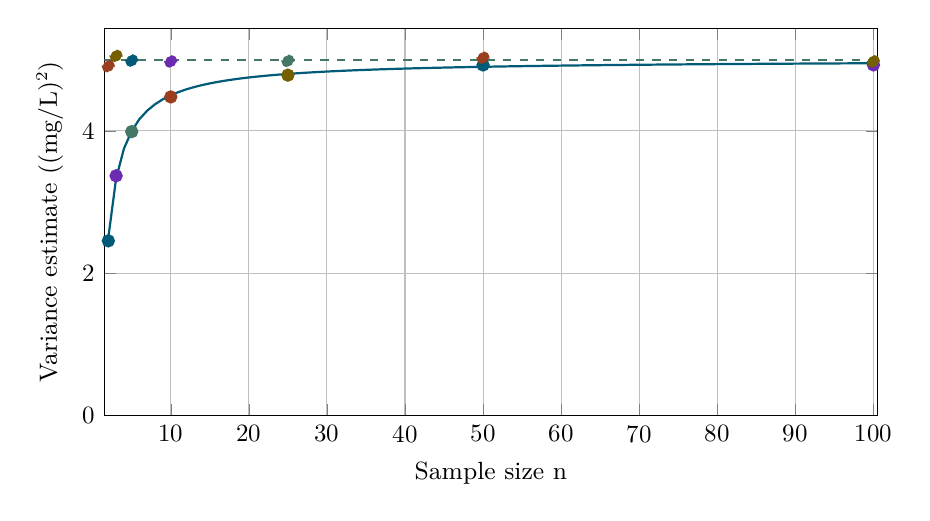
\begin{tikzpicture}
\begin{axis}[width=0.94\linewidth,
height=6.5cm,
scale only axis=false,
grid=major,
tick label style={font=\small},
label style={font=\small},
xlabel={Sample size n},
ylabel={Variance estimate ((mg/L)\ensuremath{{}^2})},
legend style={font=\footnotesize,draw=none,at={(0.5,-0.28)},anchor=north,legend columns=1,text width=0.85\linewidth,align=left},
unbounded coords=jump,
scaled ticks=false,
ymin=0,
ymax=5.442080175,
xmin=1.5,
xmax=100.5]
\addplot[color=pcd1,thick,only marks,mark=*] coordinates {(2,2.454306)};
\addplot[color=pcd2,thick,only marks,mark=*] coordinates {(3,3.368247)};
\addplot[color=pcd3,thick,only marks,mark=*] coordinates {(5,3.989123)};
\addplot[color=pcd4,thick,only marks,mark=*] coordinates {(10,4.476612)};
\addplot[color=pcd5,thick,only marks,mark=*] coordinates {(25,4.782485)};
\addplot[color=pcd1,thick,only marks,mark=*] coordinates {(50,4.925768)};
\addplot[color=pcd2,thick,only marks,mark=*] coordinates {(100,4.926258)};
\addplot[color=pcd3,thick,dashed,mark=none] coordinates {(1.5,5) (100.5,5)};
\addplot[color=pcd4,thick,dashed,only marks,mark=*] coordinates {(2,4.908612)};
\addplot[color=pcd5,thick,dashed,only marks,mark=*] coordinates {(3,5.0523705)};
\addplot[color=pcd1,thick,dashed,only marks,mark=*] coordinates {(5,4.98640375)};
\addplot[color=pcd2,thick,dashed,only marks,mark=*] coordinates {(10,4.974013333333334)};
\addplot[color=pcd3,thick,dashed,only marks,mark=*] coordinates {(25,4.981755208333333)};
\addplot[color=pcd4,thick,dashed,only marks,mark=*] coordinates {(50,5.02629387755102)};
\addplot[color=pcd5,thick,dashed,only marks,mark=*] coordinates {(100,4.976018181818182)};
\addplot[color=pcd1,thick,mark=none] coordinates {(2,2.5) (3,3.333333333333) (4,3.75) (5,4) (6,4.166666666667) (7,4.285714285714) (8,4.375) (9,4.444444444444) (10,4.5) (11,4.545454545455) (12,4.583333333333) (13,4.615384615385) (14,4.642857142857) (15,4.666666666667) (16,4.6875) (17,4.705882352941) (18,4.722222222222) (19,4.736842105263) (20,4.75) (21,4.761904761905) (22,4.772727272727) (23,4.782608695652) (24,4.791666666667) (25,4.8) (26,4.807692307692) (27,4.814814814815) (28,4.821428571429) (29,4.827586206897) (30,4.833333333333) (31,4.838709677419) (32,4.84375) (33,4.848484848485) (34,4.852941176471) (35,4.857142857143) (36,4.861111111111) (37,4.864864864865) (38,4.868421052632) (39,4.871794871795) (40,4.875) (41,4.878048780488) (42,4.880952380952) (43,4.883720930233) (44,4.886363636364) (45,4.888888888889) (46,4.891304347826) (47,4.893617021277) (48,4.895833333333) (49,4.897959183673) (50,4.9) (51,4.901960784314) (52,4.903846153846) (53,4.905660377358) (54,4.907407407407) (55,4.909090909091) (56,4.910714285714) (57,4.912280701754) (58,4.913793103448) (59,4.915254237288) (60,4.916666666667) (61,4.918032786885) (62,4.91935483871) (63,4.920634920635) (64,4.921875) (65,4.923076923077) (66,4.924242424242) (67,4.925373134328) (68,4.926470588235) (69,4.927536231884) (70,4.928571428571) (71,4.929577464789) (72,4.930555555556) (73,4.931506849315) (74,4.932432432432) (75,4.933333333333) (76,4.934210526316) (77,4.935064935065) (78,4.935897435897) (79,4.936708860759) (80,4.9375) (81,4.938271604938) (82,4.939024390244) (83,4.939759036145) (84,4.940476190476) (85,4.941176470588) (86,4.941860465116) (87,4.942528735632) (88,4.943181818182) (89,4.943820224719) (90,4.944444444444) (91,4.945054945055) (92,4.945652173913) (93,4.94623655914) (94,4.946808510638) (95,4.947368421053) (96,4.947916666667) (97,4.948453608247) (98,4.948979591837) (99,4.949494949495) (100,4.95)};

\end{axis}
\end{tikzpicture}
\end{center}


\medskip

\clearpage
\section{Standard deviation describes precision on the measurement scale}
Taking the square root of sample variance gives the sample standard deviation (\hyperref[material-3c51bc059aa86a40a69ef58bf561f7919cc39ded6ec86dc5b7a71ace70ea191f]{Eq.~\ref*{material-3c51bc059aa86a40a69ef58bf561f7919cc39ded6ec86dc5b7a71ace70ea191f}}). Its unit matches the original observations, so the interpretation in \hyperref[material-498574d44977f120c773e8d7e7132f9f650601fb3715f0c84828e6f9de00a284]{Eq.~\ref*{material-498574d44977f120c773e8d7e7132f9f650601fb3715f0c84828e6f9de00a284}} can be expressed directly on the measurement scale. The summary table in \hyperref[material-b655243aefc3b3a2e1d72aa0e7e51000f8a848919248697da8223b5cd53149e1]{Table~\ref*{material-b655243aefc3b3a2e1d72aa0e7e51000f8a848919248697da8223b5cd53149e1}} keeps variance and standard deviation connected while distinguishing their units.


\par\medskip
\Needspace{8\baselineskip}
\refstepcounter{equation}\label{material-3c51bc059aa86a40a69ef58bf561f7919cc39ded6ec86dc5b7a71ace70ea191f}
\noindent\textbf{Eq.~\ref*{material-3c51bc059aa86a40a69ef58bf561f7919cc39ded6ec86dc5b7a71ace70ea191f}.} Sample standard deviation as the square root of sample variance, in the original measurement unit.\par\nopagebreak
\paragraph{Concentration \ensuremath{\to} Variance \ensuremath{\to} Standard deviation}
\begin{center}\begin{adjustbox}{max width=\linewidth}$\displaystyle s_A^2=\frac{13}{3}\;(\mathrm{mg/L})^2$\end{adjustbox}\end{center}
\noindent\textbf{Take the nonnegative square root} (Mathematical implication)\par
Standard deviation is the nonnegative square root of variance. Taking the square root also restores the original physical unit. It is not the mean absolute deviation, and an unbiased variance estimate does not imply an unbiased square root.
\begin{center}\begin{adjustbox}{max width=\linewidth}$\displaystyle s=\sqrt{s^2}$\end{adjustbox}\end{center}

Series A has sample variance 13/3 (mg/L)\ensuremath{{}^2}.
Take its nonnegative square root: \ensuremath{\sqrt{\vphantom{x}}}(13/3) \ensuremath{\approx} 2.081666, reported here as 2.082 mg/L. The concentration unit is no longer squared.
This is a root-mean-square measure of residual size with the stated divisor, not an arithmetic mean of absolute distances.
\begin{center}\begin{adjustbox}{max width=\linewidth}$\displaystyle s_A=\sqrt{\frac{13}{3}}\;\mathrm{mg/L}\approx2.082\;\mathrm{mg/L}$\end{adjustbox}\end{center}


\begin{center}\begin{adjustbox}{max width=\linewidth}$\displaystyle s_A=\sqrt{\frac{13}{3}}\;\mathrm{mg/L}\approx2.082\;\mathrm{mg/L}$\end{adjustbox}\end{center}

\paragraph{Symbols}
\par\noindent\textbf{\(s\)} sample standard deviation
\par\noindent\textbf{\(s^2\)} Sample variance, residual sum of squares divided by n minus one for the usual mean-fitted iid estimator.
\par\noindent\textbf{\(\sqrt{\phantom{x}}\)} Nonnegative square root.
\medskip

\par\medskip
\noindent\begin{minipage}{\linewidth}
\refstepcounter{equation}\label{material-498574d44977f120c773e8d7e7132f9f650601fb3715f0c84828e6f9de00a284}
\noindent\textbf{Eq.~\ref*{material-498574d44977f120c773e8d7e7132f9f650601fb3715f0c84828e6f9de00a284}.} Authored interpretation of standard deviation on the observed measurement scale.\par\nopagebreak
\begin{center}\begin{adjustbox}{max width=\linewidth}$\displaystyle s=\sqrt{\frac{\sum_{i=1}^{n}(x_i-\bar{x})^2}{n-1}}$\end{adjustbox}\end{center}

\par\noindent\textbf{Symbols}

\par\noindent\textbf{\(i\)} Observation index, running from 1 to the declared observation count.

\par\noindent\textbf{\(n\)} number of observations in the sample

\par\noindent\textbf{\(s\)} sample standard deviation

\par\noindent\textbf{\(x_i\)} i-th observed value

\par\noindent\textbf{\(\bar{x}\)} sample arithmetic mean

\par\noindent\textbf{\(\sum\)} Sum over the indexed observations.

\par\noindent\textbf{\(\sqrt{\phantom{x}}\)} Nonnegative square root.

\end{minipage}\par
\medskip

\par\medskip
\Needspace{8\baselineskip}
\refstepcounter{scripttable}\label{material-b655243aefc3b3a2e1d72aa0e7e51000f8a848919248697da8223b5cd53149e1}
\noindent\textbf{Table~\ref*{material-b655243aefc3b3a2e1d72aa0e7e51000f8a848919248697da8223b5cd53149e1}.} Location and dispersion summaries with their respective units.\par\nopagebreak
\begin{longtable}{@{}p{\dimexpr0.333333\linewidth-2\tabcolsep\relax}p{\dimexpr0.333333\linewidth-2\tabcolsep\relax}p{\dimexpr0.333333\linewidth-2\tabcolsep\relax}@{}}
Summary & A & B \\ \hline
\endhead
Mean (mg/L) & 32/3 \ensuremath{\approx} 10.667 & 32/3 \ensuremath{\approx} 10.667 \\ \hline
MSD ((mg/L)\ensuremath{{}^2}) & 26/9 \ensuremath{\approx} 2.889 & 218/9 \ensuremath{\approx} 24.222 \\ \hline
s\ensuremath{{}^2} ((mg/L)\ensuremath{{}^2}) & 13/3 \ensuremath{\approx} 4.333 & 109/3 \ensuremath{\approx} 36.333 \\ \hline
s (mg/L) & 2.082 & 6.028 \\ \hline
\end{longtable}
\medskip

The optional sources in \hyperref[material-36ebd43e20724cd4116eee752405c566964531ada36600a40d79fcc6ccf778d7]{Listing~\ref*{material-36ebd43e20724cd4116eee752405c566964531ada36600a40d79fcc6ccf778d7}} and \hyperref[material-15d291a899596288f552acdfc94beaa37975ec37b690ca20c087ceeda307d7cc]{Listing~\ref*{material-15d291a899596288f552acdfc94beaa37975ec37b690ca20c087ceeda307d7cc}} reproduce the calculations. For quality-control repeats, the observations in \hyperref[material-264aa60c25b8cbee43eaac5351798b73b5dccd8f404892218dff8ae28fc57fa3]{Table~\ref*{material-264aa60c25b8cbee43eaac5351798b73b5dccd8f404892218dff8ae28fc57fa3}} describe precision under the repeated conditions. The target illustration in \hyperref[material-5c3b7ab3fdcd1cd9b6341789e63f91e1e44e5645bf2d42ae49594690be0b705b]{Fig.~\ref*{material-5c3b7ab3fdcd1cd9b6341789e63f91e1e44e5645bf2d42ae49594690be0b705b}} contrasts narrower and wider scatter around a deliberately chosen reference centre. Assessing trueness additionally requires evidence connecting the method's expectation with an appropriate reference value.


\par\medskip
\Needspace{8\baselineskip}
\refstepcounter{listing}\label{material-36ebd43e20724cd4116eee752405c566964531ada36600a40d79fcc6ccf778d7}
\noindent\textbf{Listing~\ref*{material-36ebd43e20724cd4116eee752405c566964531ada36600a40d79fcc6ccf778d7}.} Optional R reproduction of the variance calculation.\par\nopagebreak
\begin{Verbatim}[fontsize=\footnotesize,breaklines=true,breakanywhere=true]
a <- c(9, 10, 13)
b <- c(5, 10, 17)
mean_a <- mean(a)
mean_b <- mean(b)
c(mean_a, mean_b)
\end{Verbatim}

\par\noindent\textbf{c(...)}

Combines values into a vector; also collects results for output.

\par\noindent\textbf{mean(x)}

Calculates the arithmetic mean of the values in x.

\par\noindent\textbf{name <- value}

Assignment operator: stores a value under a name.

\medskip

\par\medskip
\Needspace{8\baselineskip}
\refstepcounter{listing}\label{material-15d291a899596288f552acdfc94beaa37975ec37b690ca20c087ceeda307d7cc}
\noindent\textbf{Listing~\ref*{material-15d291a899596288f552acdfc94beaa37975ec37b690ca20c087ceeda307d7cc}.} Optional R reproduction of the standard-deviation calculation.\par\nopagebreak
\begin{Verbatim}[fontsize=\footnotesize,breaklines=true,breakanywhere=true]
a <- c(9, 10, 13)
b <- c(5, 10, 17)
va <- var(a)
vb <- var(b)
sa <- sd(a)
sb <- sd(b)
c(va, vb, sa, sb)
\end{Verbatim}

\par\noindent\textbf{c(...)}

Combines input values or collects output results into a vector.

\par\noindent\textbf{var(x)}

Calculates sample variance using divisor n\ensuremath{-}1.

\par\noindent\textbf{sd(x)}

Calculates sample SD, the square root of var(x).

\medskip

\par\medskip
\Needspace{8\baselineskip}
\refstepcounter{scripttable}\label{material-264aa60c25b8cbee43eaac5351798b73b5dccd8f404892218dff8ae28fc57fa3}
\noindent\textbf{Table~\ref*{material-264aa60c25b8cbee43eaac5351798b73b5dccd8f404892218dff8ae28fc57fa3}.} Five quality-control repeats per method, with their means and sample standard deviations in mg/L.\par\nopagebreak
\begin{longtable}{@{}p{\dimexpr0.250000\linewidth-2\tabcolsep\relax}p{\dimexpr0.250000\linewidth-2\tabcolsep\relax}p{\dimexpr0.250000\linewidth-2\tabcolsep\relax}p{\dimexpr0.250000\linewidth-2\tabcolsep\relax}@{}}
Method & Values & Mean & SD \\ \hline
\endhead
A & 9.8, 10.0, 10.1, 9.9, 10.2 & 10.000 & 0.158 \\ \hline
B & 8.7, 10.8, 9.5, 11.2, 9.8 & 10.000 & 1.007 \\ \hline
\end{longtable}
\medskip

\par\medskip
\Needspace{10cm}
\refstepcounter{figure}\label{material-5c3b7ab3fdcd1cd9b6341789e63f91e1e44e5645bf2d42ae49594690be0b705b}
\noindent\textbf{Fig.~\ref*{material-5c3b7ab3fdcd1cd9b6341789e63f91e1e44e5645bf2d42ae49594690be0b705b}.} Illustrative target patterns centred by construction: crosses have smaller spread and open circles have larger spread. The coordinates are schematic.\par\nopagebreak
\begin{center}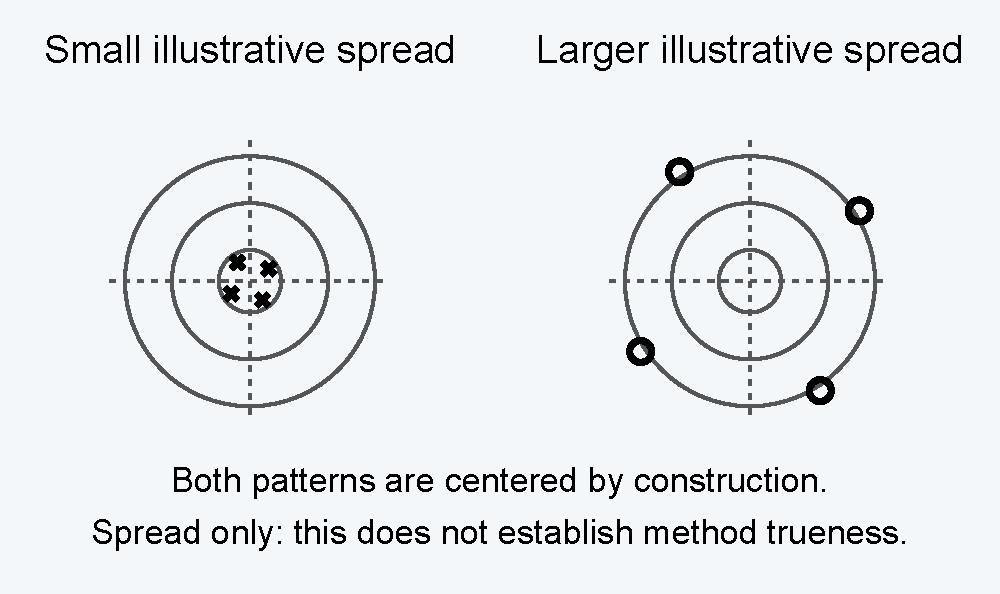
\includegraphics[width=\linewidth,height=.62\textheight,keepaspectratio]{asset-cbdea70d3ad070935edeb09a07924400642366fd46638cfc2b44ec80c2aa3aa5.pdf}\end{center}

\medskip

The shifted-data comparison in \hyperref[material-f809a61da8b90676cb2b1826cd8e39325c7989eac78586e69f3ec92ca906da64]{Fig.~\ref*{material-f809a61da8b90676cb2b1826cd8e39325c7989eac78586e69f3ec92ca906da64}} clarifies that location and spread are complementary. A common shift changes the mean while preserving distances between observations and their centre. Consequently, a precision statement identifies the measurement conditions and the variation it summarizes; a broader quality statement also addresses calibration, reference values and possible systematic effects.


\par\medskip
\Needspace{10cm}
\refstepcounter{figure}\label{material-f809a61da8b90676cb2b1826cd8e39325c7989eac78586e69f3ec92ca906da64}
\noindent\textbf{Fig.~\ref*{material-f809a61da8b90676cb2b1826cd8e39325c7989eac78586e69f3ec92ca906da64}.} A common shift changes the location of the authored observations while retaining their spread.\par\nopagebreak
\begin{center}
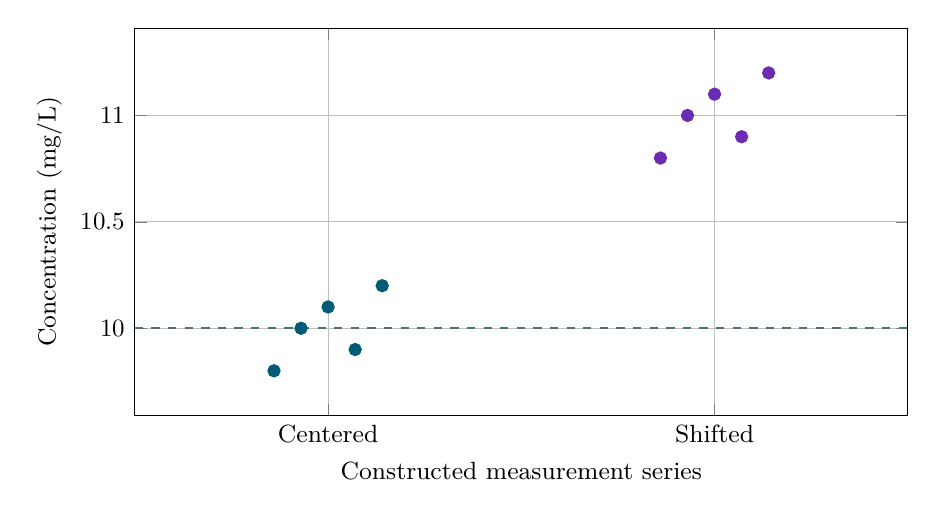
\begin{tikzpicture}
\begin{axis}[width=0.94\linewidth,
height=6.5cm,
scale only axis=false,
grid=major,
tick label style={font=\small},
label style={font=\small},
xlabel={Constructed measurement series},
ylabel={Concentration (mg/L)},
legend style={font=\footnotesize,draw=none,at={(0.5,-0.28)},anchor=north,legend columns=1,text width=0.85\linewidth,align=left},
unbounded coords=jump,
scaled ticks=false,
ymin=9.590000000000002,
ymax=11.409999999999998,
xmin=0.5,
xmax=2.5,
xtick={1,2},
xticklabels={{Centered},{Shifted}}]
\addplot[color=pcd1,thick,only marks,mark=*] coordinates {(0.86,9.8) (0.9299999999999999,10) (1,10.1) (1.07,9.9) (1.1400000000000001,10.2)};
\addplot[color=pcd2,thick,only marks,mark=*] coordinates {(1.8599999999999999,10.8) (1.93,11) (2,11.1) (2.07,10.9) (2.14,11.2)};
\addplot[color=pcd3,thick,dashed,mark=none] coordinates {(0.5,10) (2.5,10)};

\end{axis}
\end{tikzpicture}
\end{center}


\medskip

\clearpage
\section{Match the spread estimate to the repeated stage of the procedure}
A measurement result can vary because of several stages: collection, preparation and instrument reading. The process diagram in \hyperref[material-bd5fae09df53bb9f43f20ce5f9835de038186c4315e12d3510c598e0fdb85f42]{Fig.~\ref*{material-bd5fae09df53bb9f43f20ce5f9835de038186c4315e12d3510c598e0fdb85f42}} identifies the authored stages. Repeating a reading of one preparation represents a different experiment from preparing new portions or returning to new sampling sites.


\par\medskip
\Needspace{10cm}
\refstepcounter{figure}\label{material-bd5fae09df53bb9f43f20ce5f9835de038186c4315e12d3510c598e0fdb85f42}
\noindent\textbf{Fig.~\ref*{material-bd5fae09df53bb9f43f20ce5f9835de038186c4315e12d3510c598e0fdb85f42}.} Measurement-process stages used to identify the scope of replication and variation components.\par\nopagebreak
\par\medskip\noindent\textcolor{pcd1}{\textbf{1. Sampling site}}\par
Between-site variation

\par\noindent $\longrightarrow$ 2. collect
\par\medskip\noindent\textcolor{pcd2}{\textbf{2. Independent sample}}\par
Between samples within a site

\par\noindent $\longrightarrow$ 3. prepare
\par\medskip\noindent\textcolor{pcd3}{\textbf{3. Sample preparation}}\par
Between preparations of a sample

\par\noindent $\longrightarrow$ 4. measure
\par\medskip\noindent\textcolor{pcd4}{\textbf{4. Instrument repeat}}\par
Instrumental replicates within a preparation


\medskip

The component model in \hyperref[material-19cc90194bfdbfe7309e2d21faa0a09ac6ebe8d0dee1107046da41d0e3c2c632]{Eq.~\ref*{material-19cc90194bfdbfe7309e2d21faa0a09ac6ebe8d0dee1107046da41d0e3c2c632}} describes how the relevant variance contributions combine under its stated assumptions. Converting the combined variance to standard deviation gives \hyperref[material-1e06c0942fae34acf860bf8ae41141cf147fbcc8369e592fe4eeda99e47a8cde]{Eq.~\ref*{material-1e06c0942fae34acf860bf8ae41141cf147fbcc8369e592fe4eeda99e47a8cde}}. Variances add for the specified uncorrelated components; standard deviations combine through the corresponding square-root calculation. A design with dependence requires its covariance structure to be included.


\par\medskip
\Needspace{8\baselineskip}
\refstepcounter{equation}\label{material-19cc90194bfdbfe7309e2d21faa0a09ac6ebe8d0dee1107046da41d0e3c2c632}
\noindent\textbf{Eq.~\ref*{material-19cc90194bfdbfe7309e2d21faa0a09ac6ebe8d0dee1107046da41d0e3c2c632}.} Variance-component combination with the complete authored assumptions and notation.\par\nopagebreak
\paragraph{Combining independent analytical variance contributions}
\begin{center}\begin{adjustbox}{max width=\linewidth}$\displaystyle \sigma_{\mathrm{total}}^2=\operatorname{Var}(A+B+C)$\end{adjustbox}\end{center}
\noindent\textbf{Add the independent component variances} (Requires statistical assumptions)\par
For independent finite-variance contributions, covariance terms vanish. Therefore Var(A+B) = Var(A)+Var(B), and the finite-sum extension gives total variance as the sum of component variances. For correlated sources Var(A+B) also contains 2 Cov(A,B). This law concerns an assumed model, not differences between pooled experimental SDs.
\begin{center}\begin{adjustbox}{max width=\linewidth}$\displaystyle \begin{gathered}\operatorname{Var}(A+B)=\operatorname{Var}(A)+\operatorname{Var}(B)\\\sigma_{\mathrm{total}}^2=\sum_k\sigma_k^2\end{gathered}$\end{adjustbox}\end{center}

Treat A, B and C as additive random contributions, all expressed in mg/L. Their illustrative variances are 4, 1 and 0.25 (mg/L)\ensuremath{{}^2}.
Independence removes the covariance terms. Add the three variances to obtain 5.25 (mg/L)\ensuremath{{}^2}.
The numbers are model inputs for teaching, not variance components isolated from the lake or QC data.
\begin{center}\begin{adjustbox}{max width=\linewidth}$\displaystyle \sigma_{\mathrm{total}}^2=4+1+0.25=5.25\;(\mathrm{mg/L})^2$\end{adjustbox}\end{center}

\par\textbf{Illustrative independent additive model} Illustrative model, not estimated components: sampling variance 4, preparation variance 1, instrument variance 0.25 (mg/L)\ensuremath{{}^2}. Assume independent additive contributions with finite variance. Correlated sources require covariance terms.
\begin{center}\begin{adjustbox}{max width=\linewidth}$\displaystyle \sigma_{\mathrm{total}}^2=4+1+0.25=5.25\;(\mathrm{mg/L})^2$\end{adjustbox}\end{center}

\paragraph{Symbols}
\par\noindent\textbf{\(A\)} Additive sampling contribution in the illustrative model.
\par\noindent\textbf{\(B\)} Additive preparation contribution in the illustrative model.
\par\noindent\textbf{\(C\)} Additive instrument contribution in the illustrative model.
\par\noindent\textbf{\(\operatorname{Var}\)} Variance: expected squared deviation of a random quantity from its expectation.
\par\noindent\textbf{\(\sigma_{\mathrm{total}}^2\)} Total variance in (mg/L)\ensuremath{{}^2}.
\medskip

\par\medskip
\Needspace{8\baselineskip}
\refstepcounter{equation}\label{material-1e06c0942fae34acf860bf8ae41141cf147fbcc8369e592fe4eeda99e47a8cde}
\noindent\textbf{Eq.~\ref*{material-1e06c0942fae34acf860bf8ae41141cf147fbcc8369e592fe4eeda99e47a8cde}.} Standard deviation corresponding to the combined component variance.\par\nopagebreak
\paragraph{Combining independent analytical variance contributions}
\begin{center}\begin{adjustbox}{max width=\linewidth}$\displaystyle \sigma_{\mathrm{total}}^2=4+1+0.25=5.25\;(\mathrm{mg/L})^2$\end{adjustbox}\end{center}
\noindent\textbf{Take one square root after adding} (Mathematical implication)\par
After adding variances in the same squared unit, take one nonnegative square root. Standard deviations are not directly additive. This root-sum-of-squares calculation needs the independence/additivity assumptions used in the preceding step.
\begin{center}\begin{adjustbox}{max width=\linewidth}$\displaystyle \sigma_{\mathrm{total}}=\sqrt{\sum_k\sigma_k^2}$\end{adjustbox}\end{center}

Take one square root of the total 5.25 (mg/L)\ensuremath{{}^2}, giving approximately 2.291 mg/L.
Adding the individual SDs would give 2 + 1 + 0.5 = 3.5 mg/L, which is not the SD of this independent sum.
If contributions were correlated, include covariance terms before taking the square root.
\begin{center}\begin{adjustbox}{max width=\linewidth}$\displaystyle \sigma_{\mathrm{total}}=\sqrt{5.25}\;\mathrm{mg/L}\approx2.291\;\mathrm{mg/L}$\end{adjustbox}\end{center}

\par\textbf{Illustrative independent additive model} Illustrative model, not estimated components: sampling variance 4, preparation variance 1, instrument variance 0.25 (mg/L)\ensuremath{{}^2}. Assume independent additive contributions with finite variance. Correlated sources require covariance terms.
\begin{center}\begin{adjustbox}{max width=\linewidth}$\displaystyle \sigma_{\mathrm{total}}=\sqrt{5.25}\;\mathrm{mg/L}\approx2.291\;\mathrm{mg/L}$\end{adjustbox}\end{center}

\paragraph{Symbols}
\par\noindent\textbf{\(\sigma_{\mathrm{total}}\)} Total standard deviation in mg/L.
\par\noindent\textbf{\(\sigma_{\mathrm{total}}^2\)} Total variance in (mg/L)\ensuremath{{}^2}.
\par\noindent\textbf{\(\sqrt{\phantom{x}}\)} Nonnegative square root.
\medskip

The replication matrix in \hyperref[material-f2e977d856c3896b2203467434ef24c0095b0635787a13b0c9f8255474ed22c5]{Table~\ref*{material-f2e977d856c3896b2203467434ef24c0095b0635787a13b0c9f8255474ed22c5}} connects repeated stages with the variation they can reveal. The site comparison in \hyperref[material-ffea4585f3068b2a1a87c6f7efd933e36c399b83d8f322ad0d7a9f0024ee6f29]{Fig.~\ref*{material-ffea4585f3068b2a1a87c6f7efd933e36c399b83d8f322ad0d7a9f0024ee6f29}} adds the spatial context. Relative standard deviation (\hyperref[material-60ac04756f6cb239483defb829cfba2c03de13438576d7d52f4271c00ade8eff]{Eq.~\ref*{material-60ac04756f6cb239483defb829cfba2c03de13438576d7d52f4271c00ade8eff}}) expresses spread relative to the mean; the authored comparison in \hyperref[material-5f8c73306fb755a786981aa9669990663cbae9f069c8d4144d1e5b099b2686e2]{Table~\ref*{material-5f8c73306fb755a786981aa9669990663cbae9f069c8d4144d1e5b099b2686e2}} retains both absolute and relative information. A useful relative comparison requires a meaningful ratio scale and a reference mean sufficiently separated from zero.


\par\medskip
\Needspace{8\baselineskip}
\refstepcounter{scripttable}\label{material-f2e977d856c3896b2203467434ef24c0095b0635787a13b0c9f8255474ed22c5}
\noindent\textbf{Table~\ref*{material-f2e977d856c3896b2203467434ef24c0095b0635787a13b0c9f8255474ed22c5}.} Replication design matrix connecting repeated procedural stages with the variation represented.\par\nopagebreak
\begin{longtable}{@{}p{\dimexpr0.250000\linewidth-2\tabcolsep\relax}p{\dimexpr0.250000\linewidth-2\tabcolsep\relax}p{\dimexpr0.250000\linewidth-2\tabcolsep\relax}p{\dimexpr0.250000\linewidth-2\tabcolsep\relax}@{}}
Repeated level & Measurement structure & Readings & Included variation / shared levels \\ \hline
\endhead
Instrumental repeats & 3 injections, one vial & 3 & Instrument; preparation and field sample shared \\ \hline
Preparation repeats & 3 preparations \ensuremath{\times} 3 injections & 9 & Preparation + instrument; field sample shared \\ \hline
Field samples & 3 samples \ensuremath{\times} 3 preparations \ensuremath{\times} 3 injections & 27 & Within-site sampling + preparation + instrument; site shared \\ \hline
Sampling sites & 3 sites \ensuremath{\times} 3 samples \ensuremath{\times} 3 preparations \ensuremath{\times} 3 injections & 81 & Between-site + all downstream variation; nested readings remain dependent \\ \hline
\end{longtable}
\medskip

\par\medskip
\Needspace{10cm}
\refstepcounter{figure}\label{material-ffea4585f3068b2a1a87c6f7efd933e36c399b83d8f322ad0d7a9f0024ee6f29}
\noindent\textbf{Fig.~\ref*{material-ffea4585f3068b2a1a87c6f7efd933e36c399b83d8f322ad0d7a9f0024ee6f29}.} Site-level measurement comparison under the authored sampling and replication design.\par\nopagebreak
\begin{center}
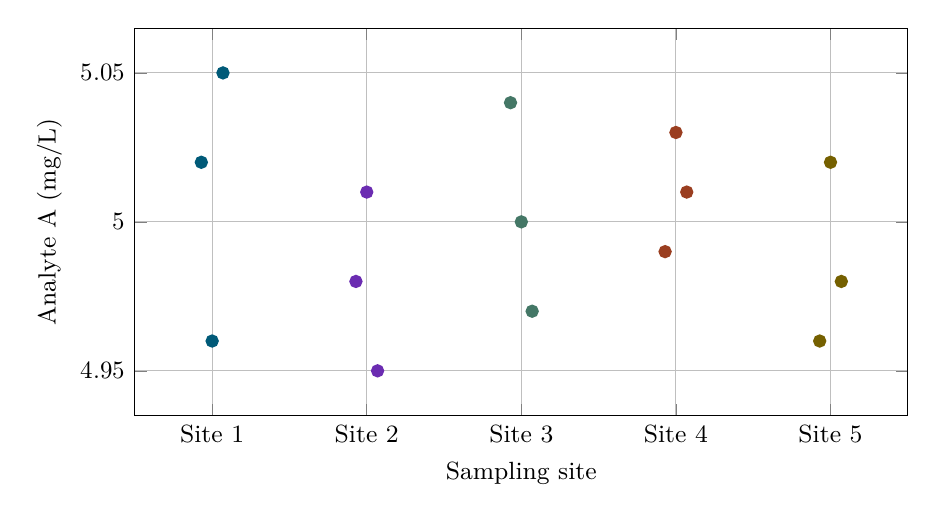
\begin{tikzpicture}
\begin{axis}[width=0.94\linewidth,
height=6.5cm,
scale only axis=false,
grid=major,
tick label style={font=\small},
label style={font=\small},
xlabel={Sampling site},
ylabel={Analyte A (mg/L)},
legend style={font=\footnotesize,draw=none,at={(0.5,-0.28)},anchor=north,legend columns=1,text width=0.85\linewidth,align=left},
unbounded coords=jump,
scaled ticks=false,
ymin=4.9350000000000005,
ymax=5.0649999999999995,
xmin=0.5,
xmax=5.5,
xtick={1,2,3,4,5},
xticklabels={{Site 1},{Site 2},{Site 3},{Site 4},{Site 5}}]
\addplot[color=pcd1,thick,only marks,mark=*] coordinates {(0.9299999999999999,5.02) (1,4.96) (1.07,5.05)};
\addplot[color=pcd2,thick,only marks,mark=*] coordinates {(1.93,4.98) (2,5.01) (2.07,4.95)};
\addplot[color=pcd3,thick,only marks,mark=*] coordinates {(2.93,5.04) (3,5) (3.07,4.97)};
\addplot[color=pcd4,thick,only marks,mark=*] coordinates {(3.93,4.99) (4,5.03) (4.07,5.01)};
\addplot[color=pcd5,thick,only marks,mark=*] coordinates {(4.93,4.96) (5,5.02) (5.07,4.98)};

\end{axis}
\end{tikzpicture}
\end{center}


\medskip

\par\medskip
\noindent\begin{minipage}{\linewidth}
\refstepcounter{equation}\label{material-60ac04756f6cb239483defb829cfba2c03de13438576d7d52f4271c00ade8eff}
\noindent\textbf{Eq.~\ref*{material-60ac04756f6cb239483defb829cfba2c03de13438576d7d52f4271c00ade8eff}.} Relative standard deviation, including the ratio-scale and denominator conventions.\par\nopagebreak
\begin{center}\begin{adjustbox}{max width=\linewidth}$\displaystyle \mathrm{RSD}=\frac{s}{|\bar{x}|},\qquad\mathrm{RSD}(\%)=100\,\frac{s}{|\bar{x}|}$\end{adjustbox}\end{center}

\par\noindent\textbf{Symbols}

\par\noindent\textbf{Spread relative to level} RSD: relative standard deviation; s: sample SD; \ensuremath{\bar{x}}: sample mean. | | takes its absolute value. The mean must be nonzero and sufficiently far from zero.

\par\noindent\textbf{Ratio or percentage} The units cancel. RSD is dimensionless. Multiplying by 100 expresses its numerical percentage; \% denotes percent. A ratio of 0.02 is 2\%.

\par\noindent\textbf{Meaningful ratios} Use a suitable ratio-scale quantity with a meaningful zero and compatible measurement conditions. A nonzero mean alone is not sufficient.

\end{minipage}\par
\medskip

\par\medskip
\Needspace{8\baselineskip}
\refstepcounter{scripttable}\label{material-5f8c73306fb755a786981aa9669990663cbae9f069c8d4144d1e5b099b2686e2}
\noindent\textbf{Table~\ref*{material-5f8c73306fb755a786981aa9669990663cbae9f069c8d4144d1e5b099b2686e2}.} Absolute and relative spread summaries for the authored comparison data.\par\nopagebreak
\begin{longtable}{@{}p{\dimexpr0.250000\linewidth-2\tabcolsep\relax}p{\dimexpr0.250000\linewidth-2\tabcolsep\relax}p{\dimexpr0.250000\linewidth-2\tabcolsep\relax}p{\dimexpr0.250000\linewidth-2\tabcolsep\relax}@{}}
Quantity & QC A (mg/L) & QC B (g/L) & QC B back in mg/L \\ \hline
\endhead
Mean & 10 & 0.010 & 10 \\ \hline
Sample SD & 0.158114 & 0.00100747 & 1.00747 \\ \hline
RSD (\%) & 1.5811 & 10.0747 & 10.0747 \\ \hline
\end{longtable}
\medskip

\clearpage
\section{Independent repetition improves the precision of an average}
The standard deviation of individual results and the standard deviation of their average refer to different random quantities. Under independent sampling with a common finite variance, the sample-mean variance derived earlier gives the population standard error in \hyperref[material-69d79584f4fa9298cc0c61b30181685088cb7740196d55b164631fdabc898d72]{Eq.~\ref*{material-69d79584f4fa9298cc0c61b30181685088cb7740196d55b164631fdabc898d72}}. Replacing the population standard deviation by its sample estimate gives \hyperref[material-3b01d7c7b582bde3f7cdc394f2fd2effd890866817d9c1b9d676ebfe63105ff2]{Eq.~\ref*{material-3b01d7c7b582bde3f7cdc394f2fd2effd890866817d9c1b9d676ebfe63105ff2}}.


\par\medskip
\noindent\begin{minipage}{\linewidth}
\refstepcounter{equation}\label{material-69d79584f4fa9298cc0c61b30181685088cb7740196d55b164631fdabc898d72}
\noindent\textbf{Eq.~\ref*{material-69d79584f4fa9298cc0c61b30181685088cb7740196d55b164631fdabc898d72}.} Population standard error of an average under the stated independent common-variance sampling model.\par\nopagebreak
\begin{center}\begin{adjustbox}{max width=\linewidth}$\displaystyle \operatorname{SE}(\bar Y)=\frac{\sigma}{\sqrt n}$\end{adjustbox}\end{center}

\par\noindent\textbf{Symbols}

\par\noindent\textbf{\(\operatorname{SE}\)} Standard error: the standard deviation of an estimator's sampling distribution. Here, random uncertainty of the sample mean under the stated sampling assumptions.

\par\noindent\textbf{\(\bar Y\)} Random sample mean of n measurements Y\_i; Y is a local renaming of the earlier measurement variable X, not a new dataset.

\par\noindent\textbf{\(n\)} number of observations in the sample

\par\noindent\textbf{\(σ\)} population standard deviation

\end{minipage}\par
\medskip

\par\medskip
\noindent\begin{minipage}{\linewidth}
\refstepcounter{equation}\label{material-3b01d7c7b582bde3f7cdc394f2fd2effd890866817d9c1b9d676ebfe63105ff2}
\noindent\textbf{Eq.~\ref*{material-3b01d7c7b582bde3f7cdc394f2fd2effd890866817d9c1b9d676ebfe63105ff2}.} Estimated standard error using the sample standard deviation.\par\nopagebreak
\begin{center}\begin{adjustbox}{max width=\linewidth}$\displaystyle \widehat{\operatorname{SE}}(\bar Y)=\frac{s}{\sqrt n}$\end{adjustbox}\end{center}

\par\noindent\textbf{Symbols}

\par\noindent\textbf{\(\bar Y\)} Random sample mean of n measurements Y\_i; Y is a local renaming of the earlier measurement variable X, not a new dataset.

\par\noindent\textbf{\(\widehat{\operatorname{SE}}\)} Estimated standard error, using the observed sample SD s in place of unknown population SD \ensuremath{\sigma}.

\par\noindent\textbf{\(n\)} number of observations in the sample

\par\noindent\textbf{\(s\)} sample standard deviation

\end{minipage}\par
\medskip

The square-root rate in \hyperref[material-acaac83e17deb45115190b443416f21f4724b0e3dc7340e558a63f59196ab0ac]{Eq.~\ref*{material-acaac83e17deb45115190b443416f21f4724b0e3dc7340e558a63f59196ab0ac}} explains why improving mean precision through repetition has diminishing returns: reducing the standard error by a given factor requires increasing the independent sample size by that factor squared. The worked example in \hyperref[material-06ae2242c81e5aac1a8cf29c600de4d91a8abb59c92e191ec76b304fc8742fe1]{Eq.~\ref*{material-06ae2242c81e5aac1a8cf29c600de4d91a8abb59c92e191ec76b304fc8742fe1}} keeps the authored units and sample size visible. The individual-result spread remains a property of the measurement conditions while the average becomes more stable.


\par\medskip
\noindent\begin{minipage}{\linewidth}
\refstepcounter{equation}\label{material-acaac83e17deb45115190b443416f21f4724b0e3dc7340e558a63f59196ab0ac}
\noindent\textbf{Eq.~\ref*{material-acaac83e17deb45115190b443416f21f4724b0e3dc7340e558a63f59196ab0ac}.} Square-root sample-size relationship for mean precision under the authored assumptions.\par\nopagebreak
\begin{center}\begin{adjustbox}{max width=\linewidth}$\displaystyle \begin{gathered}\operatorname{SE}_n=\frac{\sigma}{\sqrt n}\quad\xrightarrow[n\to\infty]{}0\\\operatorname{SE}_{4n}=\frac12\operatorname{SE}_n\end{gathered}$\end{adjustbox}\end{center}

\par\noindent\textbf{Symbols}

\par\noindent\textbf{\(\operatorname{SE}\)} Standard error: the standard deviation of an estimator's sampling distribution. Here, random uncertainty of the sample mean under the stated sampling assumptions.

\par\noindent\textbf{\(n\)} number of observations in the sample

\par\noindent\textbf{\(σ\)} population standard deviation

\end{minipage}\par
\medskip

\par\medskip
\noindent\begin{minipage}{\linewidth}
\refstepcounter{equation}\label{material-06ae2242c81e5aac1a8cf29c600de4d91a8abb59c92e191ec76b304fc8742fe1}
\noindent\textbf{Eq.~\ref*{material-06ae2242c81e5aac1a8cf29c600de4d91a8abb59c92e191ec76b304fc8742fe1}.} Worked standard-error calculation with the authored sample size and measurement units.\par\nopagebreak
\begin{center}\begin{adjustbox}{max width=\linewidth}$\displaystyle \begin{gathered}\widehat{\operatorname{SE}}(\bar Y)=\frac{0.1581}{\sqrt5}\approx0.0707\;\mathrm{mg/L}\\\boxed{\bar y\;\pm\;\widehat{\operatorname{SE}}(\bar Y)=(10.00\pm0.07)\;\mathrm{mg/L}}\end{gathered}$\end{adjustbox}\end{center}

\par\noindent\textbf{Symbols}

\par\noindent\textbf{\(\bar Y\)} Random sample mean of n measurements Y\_i; Y is a local renaming of the earlier measurement variable X, not a new dataset.

\par\noindent\textbf{\(\widehat{\operatorname{SE}}\)} Estimated standard error, using the observed sample SD s in place of unknown population SD \ensuremath{\sigma}.

\par\noindent\textbf{\(\bar y\)} Observed arithmetic mean of the same measurements, using the local Y notation.

\end{minipage}\par
\medskip

The replication comparison in \hyperref[material-4789d9e14a0774499aa44a89785d3bf07e6f9118a2cf2c5ca9489f1b894fb2e5]{Fig.~\ref*{material-4789d9e14a0774499aa44a89785d3bf07e6f9118a2cf2c5ca9489f1b894fb2e5}} and optional source in \hyperref[material-05a5d233553d6bb58d52868356fbf9d4c2bb4664730260a9af2718fb1e3eb8de]{Listing~\ref*{material-05a5d233553d6bb58d52868356fbf9d4c2bb4664730260a9af2718fb1e3eb8de}} connect this rate with design choices. Shared preparation effects or correlated readings change the effective information gained by repetition. Reporting an uncertainty for an average therefore identifies the repeated unit and its dependence assumptions. The next descriptive step examines distribution shape, because equal centres and spreads can still accompany different patterns of observations.


\par\medskip
\Needspace{10cm}
\refstepcounter{figure}\label{material-4789d9e14a0774499aa44a89785d3bf07e6f9118a2cf2c5ca9489f1b894fb2e5}
\noindent\textbf{Fig.~\ref*{material-4789d9e14a0774499aa44a89785d3bf07e6f9118a2cf2c5ca9489f1b894fb2e5}.} Authored replication comparison illustrating the information gained by the specified repeated measurements.\par\nopagebreak
\begin{center}
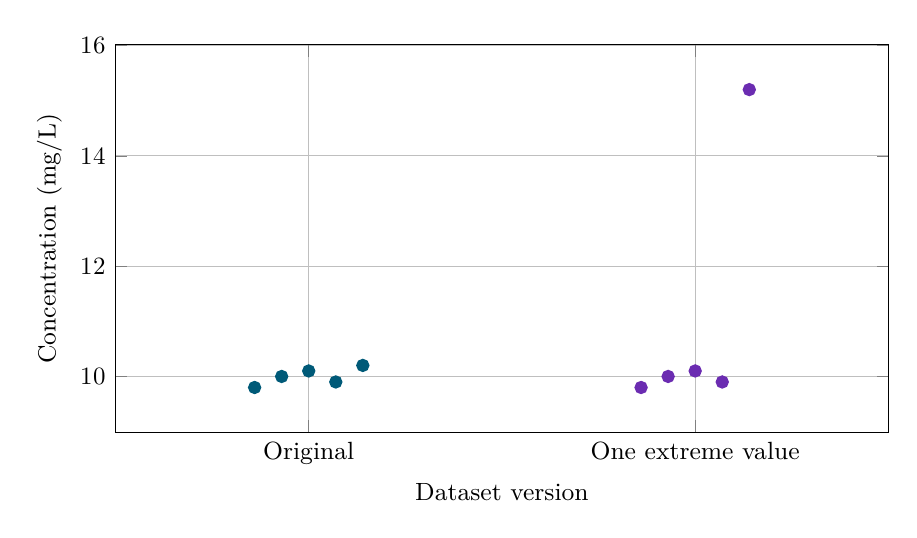
\begin{tikzpicture}
\begin{axis}[width=0.94\linewidth,
height=6.5cm,
scale only axis=false,
grid=major,
tick label style={font=\small},
label style={font=\small},
xlabel={Dataset version},
ylabel={Concentration (mg/L)},
legend style={font=\footnotesize,draw=none,at={(0.5,-0.28)},anchor=north,legend columns=1,text width=0.85\linewidth,align=left},
unbounded coords=jump,
scaled ticks=false,
ymin=8.99,
ymax=16.009999999999998,
xmin=0.5,
xmax=2.5,
xtick={1,2},
xticklabels={{Original},{One extreme value}}]
\addplot[color=pcd1,thick,only marks,mark=*] coordinates {(0.86,9.8) (0.9299999999999999,10) (1,10.1) (1.07,9.9) (1.1400000000000001,10.2)};
\addplot[color=pcd2,thick,only marks,mark=*] coordinates {(1.8599999999999999,9.8) (1.93,10) (2,10.1) (2.07,9.9) (2.14,15.2)};

\end{axis}
\end{tikzpicture}
\end{center}


\medskip

\par\medskip
\Needspace{8\baselineskip}
\refstepcounter{listing}\label{material-05a5d233553d6bb58d52868356fbf9d4c2bb4664730260a9af2718fb1e3eb8de}
\noindent\textbf{Listing~\ref*{material-05a5d233553d6bb58d52868356fbf9d4c2bb4664730260a9af2718fb1e3eb8de}.} Optional R reproduction of the replication comparison.\par\nopagebreak
\begin{Verbatim}[fontsize=\footnotesize,breaklines=true,breakanywhere=true]
a <- c(9.8, 10.0, 10.1, 9.9, 10.2)
b <- c(8.7, 10.8, 9.5, 11.2, 9.8)
ma <- mean(a); mb <- mean(b)
sa <- sd(a); sb <- sd(b)
ra <- 100*sa/ma; rb <- 100*sb/mb
inside_a <- a >= 9.5 & a <= 10.5
inside_b <- b >= 9.5 & b <= 10.5
na <- sum(inside_a); nb <- sum(inside_b)
c(ma, mb, sa, sb, ra, rb, na, nb)
\end{Verbatim}

\par\noindent\textbf{c(...)}

Combines input values or collects output results into a vector.

\par\noindent\textbf{mean(x)}

Calculates the arithmetic mean of x.

\par\noindent\textbf{sd(x)}

Calculates sample SD using the corrected variance.

\par\noindent\textbf{sum(x)}

Adds values; for logical x, counts TRUE entries.

\par\noindent\textbf{>=, <= and \&}

Operators: compare to inclusive bounds; \& requires both conditions.

\medskip

\end{document}
